\documentclass[journal]{IEEEtran}

% ---------- PACKAGES ----------
\usepackage[utf8]{inputenc} % For UTF-8 encoding
\usepackage[T1]{fontenc}    % For accented characters
\usepackage{mathptmx}       % Times New Roman font
\usepackage{graphicx}       % For including images
\usepackage{float}          % For controlling float positions
\usepackage[ruled,vlined]{algorithm2e}
% \usepackage{caption}
% \usepackage{subcaption}
\usepackage{amsmath, amsfonts, amssymb} % Common math packages
\usepackage{hyperref}
\usepackage{enumitem}       % For customizable lists
\usepackage[caption=false,font=footnotesize,labelfont=sf,textfont=sf]{subfig}
% Use natbib for flexible in‑text citations (allows \citet and \citep) while keeping numeric IEEE style
% \usepackage{cite}
\usepackage[numbers,sort&compress]{natbib}
\usepackage{array}
\usepackage{balance}
\usepackage{tikz}           % For flowcharts or block diagrams
\usetikzlibrary{shapes,arrows.meta,positioning,calc,shadows,backgrounds,decorations.pathreplacing,fit,petri,arrows}
% \usetikzlibrary{shapes, arrows.meta, positioning, chains, fit, calc, shapes.geometric, shadows}
\usepackage{booktabs}       % For professional tables with \toprule, \midrule, etc.
\usepackage{multirow}       % For table cells spanning multiple rows
\usepackage{makecell}       % For better table cell formatting

% ---------- IEEEtran RECOMMENDATIONS ----------
\hyphenation{op-tical net-works semi-conduc-tor IEEE-Xplore}
\def\BibTeX{{\rm B\kern-.05em{\sc i\kern-.025em b}\kern-.08em
   T\kern-.1667em\lower.7ex\hbox{E}\kern-.125emX}}

% ---------- TITLE & AUTHOR ----------
\title{\textbf{MSAGAT-Net: Multi-Scale Temporal Adaptive Graph Attention for Efficient Spatiotemporal Epidemic Forecasting}}

% \author{
%     \IEEEauthorblockN{Author Names}
%     \IEEEauthorblockA{Institution\\
%     Email: author@institution.edu}
% }

% \markboth{IEEE Transactions on ...}{}

\author{%
  Michael Ajao-olarinoye,~\IEEEmembership{Member, IEEE}, 
  Vasile Palade,~\IEEEmembership{Senior Member, IEEE}, 
  Fei He, 
  Petra A Wark, 
  Seyed Mousavi,
  and Zindoga Mukandavire%
  \thanks{M. Ajao-olarinoye, V. Palade, F. He, and S. Mousavi are with the Centre for Computational Science and Mathematical Modelling, Coventry University, Coventry, U.K. (e-mail: olarinoyem@coventry.ac.uk).}%
  \thanks{P. A. Wark is with the Research Methods and Evaluation Unit, Research Centre for Healthcare and Communities, Coventry University, Coventry, U.K.}%
  \thanks{Z. Mukandavire is with the Institute of Applied Research and Technology, Emirates Aviation University, Dubai, United Arab Emirates.}%
}
% \markboth{IEEE Transactions on <Journal>,~Vol.~XX, No.~X, <Month>~<Year>}%
% {Ajao-olarinoye \MakeLowercase{\textit{et al.}}: <Short Paper Title>}


\markboth{IEEE Journal of ......,~Vol.~XX, No.~YY, Month~Year}{}

% ---------- DOCUMENT BEGIN ----------
\begin{document}
\maketitle

% ---------- ABSTRACT ----------
\begin{abstract}
\textbf{Background and Objective:} Accurate spatiotemporal epidemic forecasting is critical for public health preparedness and resource allocation. However, existing graph neural network (GNN) approaches face a fundamental trade-off between computational scalability and modelling capacity, limiting their deployment in real-world surveillance systems. This study introduces MSAGAT-Net, a computationally efficient multi-scale temporal graph attention network designed to address these limitations whilst maintaining high forecasting accuracy across diverse epidemic scenarios.

\textbf{Methods:} MSAGAT-Net integrates four key architectural components: (i) efficient feature extraction via depthwise separable convolutions, (ii) an Adaptive Graph Attention Module (AGAM) employing linearised attention with low-rank projections to reduce computational complexity from $O(N^2)$ to $O(N)$, featuring a novel graph bias message passing mechanism that integrates learnable spatial structure directly into the forward computation, (iii) a Multi-Scale Temporal Feature Module (MTFM) using adaptive dilated convolutions to capture dynamics across multiple temporal resolutions, and (iv) a Progressive Prediction Refinement Module (PPRM) for stable multi-horizon forecasts. We evaluated MSAGAT-Net on seven diverse datasets spanning influenza, COVID-19, and ICU bed occupancy across multiple countries, including two novel benchmarks (LTLA-COVID and NHS-ICUBeds).

\textbf{Results:} In datasets exhibiting strong spatiotemporal dependencies, MSAGAT-Net achieved state-of-the-art performance, reducing RMSE by up to 11.2\% compared to baseline methods in the Japan-Prefectures influenza dataset and attaining superior results in LTLA-Timeseries COVID-19 forecasts for short and medium-term horizons. Comprehensive ablation studies revealed a fundamental scientific insight: optimal architectural choices are disease-specific and horizon-dependent, with spatial attention becoming increasingly critical for extended influenza forecasting yet occasionally impairing short-term COVID-19 predictions.

\textbf{Conclusions:} MSAGAT-Net provides an efficient and scalable solution for spatiotemporal epidemic forecasting that balances computational efficiency with predictive accuracy. Our findings challenge conventional assumptions about model complexity, demonstrating that sophisticated temporal processing can occasionally degrade performance compared to simpler alternatives. These insights highlight the importance of adaptive, disease-specific architectures for public health decision-making and surveillance systems.
\end{abstract}

% ---------- INDEX TERMS ----------
\begin{IEEEkeywords}
Deep Learning, Graph Neural Networks, Multi-head Attention, Time Series Analysis, Epidemic Forecasting, Adaptive Graph Learning, Multi-scale Feature Fusion, Spatiotemporal Prediction
\end{IEEEkeywords}

% ---------- SECTION I: INTRODUCTION ----------
\section{Introduction}

Spatiotemporal epidemic forecasting is critical for public health systems, enabling timely decision-making and resource allocation in response to emerging infectious diseases. The COVID-19 pandemic has underscored the importance of reliable forecasting models that can adapt to rapidly changing dynamics and provide actionable insights for public health interventions \cite{ajao2023deep,da2021covid, giuliani2020modelling, verma2022temporal, ma2024reporting}. However, developing such models presents significant challenges due to the complex interplay between spatial dependencies, temporal patterns, and the inherent uncertainty in disease transmission.

Effective epidemic forecasting requires capturing both spatial dependencies (how diseases spread between interconnected regions) and temporal patterns that range from daily reporting fluctuations to seasonal epidemic waves \cite{Panja2022Epicasting, Stone2007Seasonal}. Traditional epidemiological models, while providing valuable theoretical insights, often struggle with the computational complexity required for real-time surveillance across hundreds or thousands of regions \cite{heltberg2022spatial, s25082507, DEANGELIS201583}. 

Deep learning techniques have substantially advanced epidemic forecasting across various domains, including traffic forecasting \cite{li2017diffusion, zhang2021graph}, environmental monitoring \cite{wu2018deep, lai2018modeling}, and epidemic prediction \cite{kimForecastingEpidemicSpread2025, zhiweidingBiologyInformedRecurrentNeural2023}. Studies such as \cite{ajao2023deep, zhang2021graph, wu2018deep, lai2018modeling, Ahmadini2025} have demonstrated that recurrent neural networks (RNNs), convolutional neural networks (CNNs), and graph neural networks (GNNs) improve both predictive accuracy and modelling efficiency. Graph neural networks, in particular, have shown strong potential for epidemic forecasting by effectively learning complex spatiotemporal patterns from data, outperforming traditional and other deep learning models in capturing regional heterogeneity and dynamic transmission mechanisms \cite{Kamalov2022ReviewDL, wang2019defsi}.

Despite these advances, current approaches face three fundamental limitations that prevent their deployment in real-world surveillance systems: (1) most graph attention mechanisms suffer from quadratic computational complexity, making them prohibitively expensive for national-scale surveillance involving thousands of regions; (2) existing methods typically employ fixed architectural choices for temporal processing, failing to adapt to the diverse dynamics exhibited by different diseases and forecast horizons; and (3) multi-horizon forecasting remains unstable due to error accumulation, limiting the utility of long-range forecasts essential for public health planning and resource allocation.

To address these challenges, we propose MSAGAT-Net (Multi-Scale Temporal Adaptive Graph Attention Network), a novel architecture that achieves computational efficiency whilst maintaining high forecasting accuracy across diverse epidemic scenarios. MSAGAT-Net integrates four key components: (i) an efficient feature extraction module using depthwise separable convolutions, (ii) an Adaptive Graph Attention Module (AGAM) that reduces computational complexity from $O(N^2)$ to $O(N)$ using low-rank bottleneck projections, linearised attention, and a novel graph bias message passing mechanism that integrates learnable spatial structure directly into the forward computation, (iii) a Multi-Scale Temporal Feature Module (MTFM) that captures dynamics across multiple temporal resolutions using adaptive dilated convolutions, and (iv) a Progressive Prediction Refinement Module (PPRM) that stabilises multi-horizon forecasts by combining model-based predictions with trend-based extrapolations.

Our contributions are as follows:
\begin{enumerate}
    \item We propose an efficient graph attention mechanism that reduces complexity from $O(N^2)$ to $O(N)$ through low-rank bottleneck projections and linearised attention. A novel graph bias message passing mechanism integrates learnable spatial structure directly into the forward computation, enabling the model to capture persistent inter-regional relationships whilst maintaining linear complexity.

    \item We develop an adaptive multi-scale temporal processing framework using dilated convolutions that efficiently captures epidemic dynamics across multiple temporal resolutions, from reporting fluctuations to seasonal waves.

    \item We introduce a progressive forecast refinement module that mitigates error accumulation in multi-horizon forecasting by adaptively combining model-based forecasts with trend-based extrapolations.
    
    \item We evaluate MSAGAT-Net across seven diverse epidemic datasets spanning influenza, COVID-19, and ICU bed occupancy (including two novel benchmarks: LTLA-COVID and NHS-ICUBeds), achieving up to 11.2\% RMSE reduction compared to state-of-the-art baselines. Comprehensive ablation studies reveal that optimal architectural choices are fundamentally disease-specific and horizon-dependent, demonstrating that no single architecture universally dominates across all epidemic contexts.
\end{enumerate}


% ---------- SECTION II: LITERATURE REVIEW ----------
\section{Related Work}

Epidemic forecasting has evolved from classical compartmental models to neural network architectures that capture spatial coupling and temporal heterogeneity. This section reviews (i) spatiotemporal graph learning for epidemics, including attention and transformer-based models that learn dynamic cross-regional influence, (ii) physics-informed and hybrid neural approaches that integrate compartmental priors, and (iii) multi-scale temporal modelling and multi-horizon forecasting strategies. We position MSAGAT-Net within this landscape by highlighting the efficiency limits of quadratic attention, the rigidity of fixed architectural choices, and the need for stable long-range forecasts.

\subsection{Spatiotemporal Epidemic Modelling}

The application of graph neural networks to epidemic forecasting has emerged as a dominant paradigm, fundamentally addressing limitations of traditional compartmental models that assume uniform mixing and fixed transmission parameters \cite{lijingwangCausalGNNCausalBasedGraph2022}. A comprehensive taxonomy by Liu et al. \cite{liuReviewGraphNeural2024a, wang_deepest_2024} distinguishes between statistical epidemiology models, general machine learning models, deep neural network-based time series models and spatiotemporal approaches, with different preprocessing and modelling choices, revealing distinct trade-offs between interpretability and modelling flexibility.

Spatiotemporal approaches have demonstrated remarkable success in learning complex spatiotemporal patterns directly from data. Deng et al. \cite{dengColaGNNCrosslocationAttention2020a} presented Cola-GNN, a cross-location attention-based graph neural network for long-term Influenza-Like Illness (ILI) prediction, where the dynamic cross-location attention mechanism replaced fixed geographic adjacency matrices with learnable attention weights that adapt to time-varying transmission patterns.

Building on these foundations, Xie et al. \cite{xie2022epignn} developed EpiGNN, which combines transmission risk encoding with a Region-Aware Graph Learner that explicitly models both local clustering effects and global connectivity patterns. By incorporating human mobility data into the graph learning process, EpiGNN achieved substantial improvements on multiple epidemic forecasting tasks, reducing RMSE by approximately 9.5\% compared to baseline methods.

Gao et al. \cite{gao2021stan} proposed STAN, a spatiotemporal attention network that uses graph attention mechanisms with patient electronic health records and geography-based features. Applied to COVID-19 forecasting in all US counties, STAN achieved up to 87\% lower mean square error compared to classical SIR/SEIR models, demonstrating that attention-based spatial modelling can significantly outperform traditional compartmental approaches.

Recent developments have focused on unifying spatial and temporal modelling with more sophisticated dynamic mechanisms. Han et al. \cite{han2025dygraphformer} developed DyGraphFormer, which integrates dynamic graph learning with Transformer architectures to capture evolving spatial-temporal dependencies through gated recurrent units that continuously update graph structure based on recent observations. Similarly, Pu et al. \cite{pu2024dynamic} proposed DASTGN with dual-scale attention mechanisms that adaptively fuse spatial and temporal effects at both fine and coarse-grained resolutions.

A related direction involves hybrid approaches that incorporate epidemiological knowledge into neural architectures to improve interpretability and long-range forecast stability. For example, Cao et al.~\cite{cao2022mepognn} proposed MepoGNN, which combines region-level SEIR compartmental simulators with Graph Attention Networks, transforming static travel matrices into dynamic transmission adjacency matrices. Gao et al.~\cite{gao2023evidence} introduced HOIST, using Ising spin dynamics to regularise forecasting models based on the assumption that neighbouring regions' case counts evolve in correlated patterns. While such hybrid approaches provide theoretical grounding, they often require extensive domain expertise for model specification and may struggle to capture complex non-linear dynamics that deviate from assumed mechanistic forms.

Despite these advances, current spatiotemporal approaches face two critical limitations. First, they typically employ standard attention mechanisms with quadratic $O(N^2)$ complexity, making them computationally prohibitive for large-scale regional analysis. Recent advances in efficient attention, particularly linearised attention mechanisms that reduce complexity to $O(N)$ through low-rank projection of key and value representations with fixed bottleneck dimensions \cite{wang2020linformer}, offer promising solutions, but remain largely unexplored in epidemic forecasting contexts. Second, existing approaches often fail to maintain stability in multi-horizon forecasts, as error propagation compounds over extended forecast horizons \cite{Brooks2018Nonmechanistic}.

\subsection{Multi-Scale Temporal Modelling and Multi-Horizon Forecasting}

Epidemic time series data exhibit complex, multi-scale temporal dynamics arising from a range of underlying processes. Short-term fluctuations are often driven by reporting practices, such as testing schedules and data collection delays \cite{Panja2022Epicasting}, while longer-term patterns, including seasonal waves, are shaped by environmental factors and behavioural responses to disease spread \cite{Stone2007Seasonal}. Effective multi-horizon forecasting of such data typically falls into two principal methodological categories: (1) direct forecasting, in which models forecast multiple future time steps simultaneously, and (2) iterative (or autoregressive) forecasting, where forecasts are generated sequentially and recursively at each time step \cite{Brooks2018Nonmechanistic}. Capturing these temporal dependencies across multiple scales is therefore essential for designing forecasting models that remain robust under data irregularities and regime shifts.

Direct multi-horizon models, often implemented using sequence-to-sequence architectures with LSTM or CNN components, have demonstrated effectiveness in influenza forecasting. However, these models generally require substantial training data and exhibit sensitivity to the inclusion and quality of external covariates \cite{wu2018deep, venna2019novel}. Wang et al. \cite{wang2019defsi} developed DEFSI, which integrates deep learning with compartmental models to improve long-range forecasts, but observed that performance deteriorates significantly beyond four-week horizons due to accumulating uncertainty.

Iterative strategies, while more data-efficient, are prone to error propagation across extended forecasting horizons. This inherent limitation has motivated the development of multi-module architectures designed to capture both high-frequency fluctuations and low-frequency trends simultaneously. Deng et al. \cite{dengColaGNNCrosslocationAttention2020a} addressed these challenges using dilated convolutions for multi-scale temporal feature extraction, finding that incorporating seasonal trends improved forecast stability. However, their approach relies on fixed dilation patterns that may not adapt effectively to the changing dynamics of the epidemic in different diseases and regions.

Recognising the need to represent both short-term outbreaks and long-term epidemiological waves, recent research has explored the incorporation of external data sources, including climatic variables, demographic information, and digital surveillance indicators \cite{Luo2023Interpretable, Moss_Zarebski_Dawson_Franklin_Birrell_McCaw_2020}. Although such approaches can improve long-range predictive performance, they often require extensive feature engineering and may not generalise well in heterogeneous epidemic contexts \cite{Panja2022Epicasting}. 

These limitations across spatiotemporal modelling, physics-informed approaches, and multi-scale temporal processing underscore three critical gaps in contemporary epidemic forecasting research: (1) the computational complexity of attention mechanisms, which scales quadratically with the number of regions and hinders real-time surveillance applications; (2) the rigidity of fixed architectural designs, which limits adaptability across diverse epidemic settings; and (3) the lack of stable multi-horizon forecasting capabilities required for effective public health planning. Our proposed framework, MSAGAT-Net, addresses these challenges by integrating linearised attention for computational efficiency, adaptive multi-scale temporal processing, and progressive forecast refinement to enable stable and scalable multi-horizon epidemic forecasting.


% ---------- SECTION III: METHODOLOGY ----------
\section{Methodology}


\subsection{Problem Formulation}

Let us consider $N$ geographical regions (e.g., cities, counties, states, or NHS regions in England) as nodes in a graph. Historical epidemic data are represented as $\mathbf{X} = [\mathbf{x}_1, \mathbf{x}_2, \ldots, \mathbf{x}_T] \in \mathbb{R}^{N \times T}$, where $\mathbf{x}_t \in \mathbb{R}^N$ denotes the observed values in all $N$ regions at time step $t$. Each individual element $x_{i,t}$ represents the epidemic measure (e.g. ventilator bed occupancy or positive case count) for the region $i$ at time $t$.

For each specific region $i$, its temporal sequence is represented as $\mathbf{x}^i = [x_{i,1}, x_{i,2}, \ldots, x_{i,T}] \in \mathbb{R}^T$. This dual representation allows us to analyse both the spatial patterns (across regions at a specific time) and temporal patterns (within a region across time). 

Our primary objective is to predict future epidemic values for all regions on a specific time horizon $h$ steps ahead. Formally, given the historical data up to time $t$, we want to predict:

\begin{equation}
\mathbf{x}_{t+h} = [x_{1,t+h}, x_{2,t+h}, \ldots, x_{N,t+h}]^T
\end{equation}

For practical forecasting, we employ a sliding window approach with a fixed-length lookback period $w$. At any current time step $t$, we use the most recent observations $w$ $[\mathbf{x}_{t-w+1}, \mathbf{x}_{t-w+2}, \ldots, \mathbf{x}_t]$ to predict $\mathbf{x}_{t+h}$.

The spatial relationships between regions are encoded in a graph structure $\mathcal{G} = (\mathcal{V}, \mathcal{E}, \mathbf{A})$, where $\mathcal{V} = \{v_1, v_2, \ldots, v_N\}$ represents the set of regions, $\mathcal{E} \subseteq \mathcal{V} \times \mathcal{V}$ denotes the connections between regions and $\mathbf{A} \in \mathbb{R}^{N \times N}$ is the adjacency matrix. Each element $a_{ij}$ of $\mathbf{A}$ quantifies the strength of the relationship between regions $v_i$ and $v_j$. The adjacency matrix can be constructed based on various criteria, such as geographical proximity, transportation networks, or healthcare referral patterns. For example, in the context of epidemic forecasting, the adjacency matrix can reflect the mobility patterns of individuals between regions or the referral pathways of patients between healthcare facilities.

The forecasting task can be formalised as learning a function $f$ that maps recent historical data and graph structure to future predictions.

\begin{equation}
\mathbf{x}_{t+h} = f([\mathbf{x}_{t-w+1}, \mathbf{x}_{t-w+2}, \ldots, \mathbf{x}_t], \mathcal{G}; \boldsymbol{\Theta})
\end{equation}

where $\boldsymbol{\Theta}$ represents the learnable parameters of our forecasting model.

The challenge lies in designing this function $f$ to effectively capture both spatial dependencies between regions and temporal patterns within regions, whilst remaining computationally tractable and robust to the noisy and incomplete nature of epidemic data. Our approach, detailed in the following sections, addresses this challenge through a novel neural network architecture that combines graph attention mechanisms with multi-scale processing.

\begin{figure*}[!htbp]
    \centering
    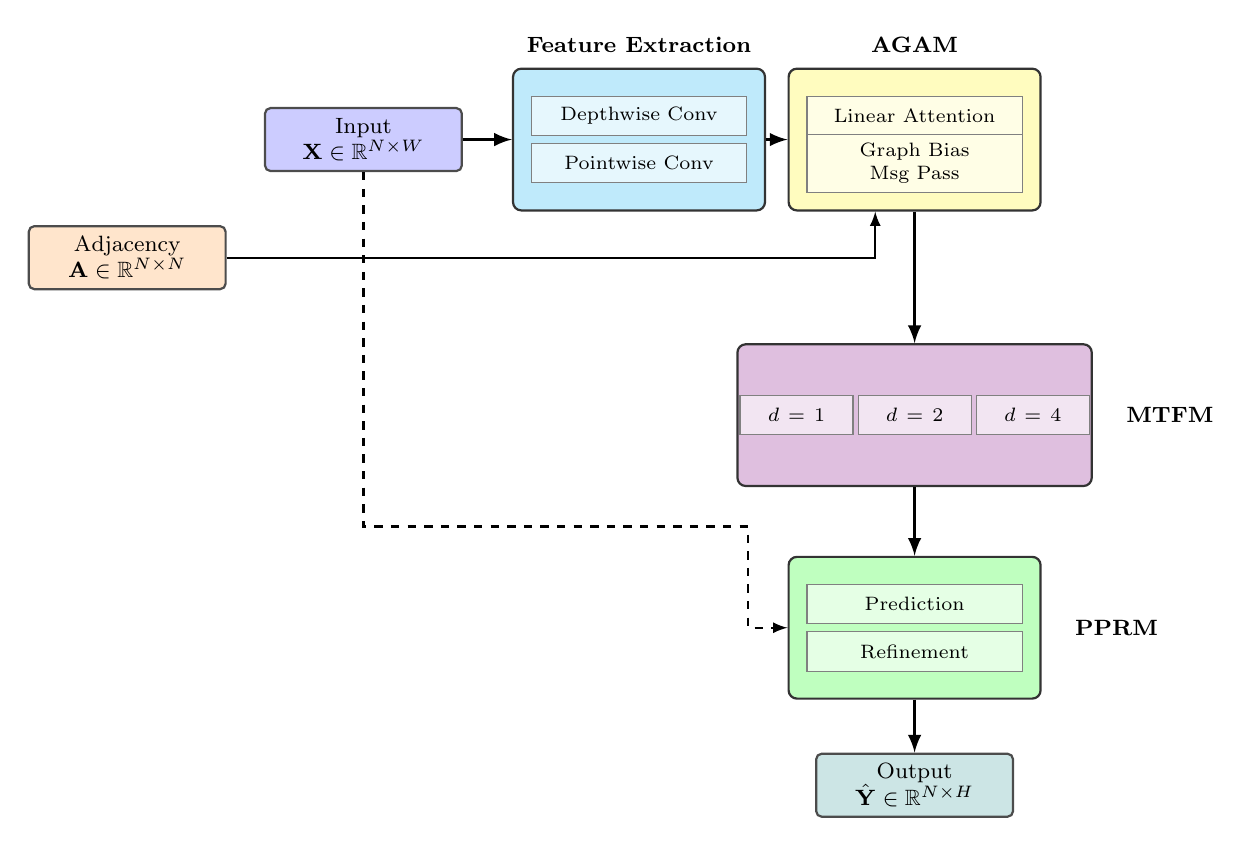
\begin{tikzpicture}[
        font=\footnotesize,
        >=latex,
        node distance = 1.5cm and 2.8cm,
        % Block styles
        module/.style={
            rectangle, 
            draw=black!80, 
            thick,
            rounded corners=3pt,
            minimum height=1.8cm, 
            minimum width=3.2cm,
            align=center,
            fill=#1!25
        },
        submodule/.style={
            rectangle, 
            draw=black!50, 
            minimum height=0.5cm, 
            text width=2.5cm,
            align=center,
            font=\scriptsize,
            fill=#1!10
        },
        data/.style={
            rectangle,
            draw=black!70,
            thick,
            rounded corners=2pt,
            minimum height=0.8cm,
            minimum width=2.5cm,
            align=center,
            fill=#1!20
        },
        arrow/.style={->, thick},
        bigarrow/.style={->, very thick},
        dashedarrow/.style={->, dashed, thick},
        label/.style={font=\footnotesize\bfseries}
    ]
    
    % Input
    \node[data=blue] (input) at (-5, 4) {Input\\$\mathbf{X} \in \mathbb{R}^{N \times W}$};
    \node[data=orange] (adj) at (-8, 2.5) {Adjacency\\$\mathbf{A} \in \mathbb{R}^{N \times N}$};
    
    % Feature Extraction
    \node[module=cyan] (feat) at (-1.5, 4) {};
    \node[label, above=2pt of feat] {Feature Extraction};
    \node[submodule=cyan] (dw) at ([yshift=0.3cm]feat.center) {Depthwise Conv};
    \node[submodule=cyan] (pw) at ([yshift=-0.3cm]feat.center) {Pointwise Conv};
    
    % AGAM
    \node[module=yellow] (agam) at (2, 4) {};
    \node[label, above=2pt of agam] {AGAM};
    \node[submodule=yellow] (attn) at ([yshift=0.3cm]agam.center) {Linear Attention};
    \node[submodule=yellow] (bias) at ([yshift=-0.3cm]agam.center) {Graph Bias Msg Pass};

    % MTFM
    \node[module=violet, minimum width=4.5cm] (mtfm) at (2.0, 0.5) {};
    \node[label, above=2pt, right=0.3cm of mtfm] {MTFM};
    \node[submodule=violet, text width=1.2cm] (s1) at ([xshift=-1.5cm]mtfm.center) {$d=1$};
    \node[submodule=violet, text width=1.2cm] (s2) at ([xshift=0cm]mtfm.center) {$d=2$};
    \node[submodule=violet, text width=1.2cm] (s3) at ([xshift=1.5cm]mtfm.center) {$d=4$};
    
    % PPRM
    \node[module=green] (ppm) at (2.0, -2.2) {};
    \node[label, above=2pt, right=0.3cm of ppm] {PPRM};
    \node[submodule=green] (pred) at ([yshift=0.3cm]ppm.center) {Prediction};
    \node[submodule=green] (refine) at ([yshift=-0.3cm]ppm.center) {Refinement};
    
    % Output
    \node[data=teal] (output) at (2.0, -4.2) {Output\\$\hat{\mathbf{Y}} \in \mathbb{R}^{N \times H}$};
    
    % Connections
    \draw[bigarrow] (input) -- (feat);
    \draw[bigarrow] (feat) -- (agam);
    \draw[bigarrow] (agam) -- (mtfm);
    \draw[bigarrow] (mtfm) -- (ppm);
    \draw[bigarrow] (ppm) -- (output);
    
    \draw[arrow] (adj) -| ([xshift=-0.5cm]agam.south);
    \draw[dashedarrow] (input) |- ([yshift=-4.5cm]input.south) -| ([xshift=-0.5cm]ppm.west) -- (ppm);
    
    \end{tikzpicture}
    \caption{Overview of the MSAGAT-Net architecture. The model processes input through four main modules: Feature Extraction (depthwise separable convolutions), AGAM, MTFM (dilation rates $d \in \{1,2,4\}$), and PPRM. The dashed line represents the skip connection for refinement.}
    \label{fig:msagat_net_architecture}
\end{figure*}

\subsection{Feature Extraction}

The first component of the MSAGAT-Net architecture is the feature extraction module, which transforms the raw time-series data into meaningful feature representations whilst maintaining computational efficiency. Given the input time-series data $\mathbf{X} = [\mathbf{x}_{t-w+1}, \mathbf{x}_{t-w+2}, \ldots, \mathbf{x}_t] \in \mathbb{R}^{N \times w}$ for the $N$ regions over a lookback window of $w$ time steps, we need to extract features that capture relevant temporal patterns for each region. This is achieved through a combination of depthwise separable convolutions and low-rank projections, which allow for efficient feature extraction while reducing the risk of overfitting. The idea of using depthwise separable convolutions is inspired by the success of this approach in computer vision tasks, where it has been shown to significantly reduce the number of parameters and computational complexity while maintaining high performance \cite{chollet2017xception}. Our adaptation of this technique draws from the work of \cite{li2023multi} and \cite{yu2022traffic}, who have successfully applied depthwise separable convolutions to feature extraction rather than the standard convolutional approach. This allows us to efficiently capture the temporal dynamics of epidemic data without incurring the high computational costs associated with traditional convolutional architectures.

\subsubsection{Depthwise Separable Convolutions}

We employ the depthwise separable convolutions to extract temporal features efficiently. This approach significantly reduces the computational complexity and number of parameters whilst maintaining expressive power. The depthwise separable convolution consists of two stages:

For each region's time-series $\mathbf{x}^i \in \mathbb{R}^w$, the depthwise convolution applies a separate filter to each input channel (in this case, we treat the time-series as a single-channel input):

\begin{equation}
\mathbf{z}^i_{\text{depth}} = \text{Conv1D}_{\text{depth}}(\mathbf{x}^i; \boldsymbol{\Theta}_{\text{depth}})
\end{equation}

where $\mathbf{z}^i_{\text{depth}} \in \mathbb{R}^{w \times d_{\text{mid}}}$ represents the intermediate features after depthwise convolution, and $d_{\text{mid}}$ is the number of intermediate feature channels.

Following the depthwise convolution, a pointwise convolution (implemented as a 1×1 convolution) is applied to combine the features across channels:

\begin{equation}
\mathbf{z}^i_{\text{point}} = \text{Conv1D}_{\text{point}}(\mathbf{z}^i_{\text{depth}}; \boldsymbol{\Theta}_{\text{point}})
\end{equation}

where $\mathbf{z}^i_{\text{point}} \in \mathbb{R}^{w \times d_{\text{feat}}}$ represents the features after pointwise convolution, and $d_{\text{feat}}$ is the number of channels of output feature.

This decomposition significantly reduces the computational complexity and number of parameters compared to standard convolutions whilst maintaining similar expressive power. Specifically, for a standard convolution with kernel size $k$, input channels $c_{\text{in}}$, and output channels $c_{\text{out}}$, the parameter count is $k \times c_{\text{in}} \times c_{\text{out}}$. In contrast, the separable convolution in depth requires only $k \times c_{\text{in}} + c_{\text{in}} \times c_{\text{out}}$ parameters.

After each convolutional operation, we apply batch normalisation followed by ReLU activation to enhance training stability and introduce non-linearity:

\begin{equation}
\mathbf{z}^i_{\text{norm}} = \text{ReLU}(\text{BatchNorm}(\mathbf{z}^i_{\text{point}}))
\end{equation}

This normalisation step helps mitigate internal covariate shift during training, whilst the non-linear activation enables the model to capture complex temporal patterns in the epidemic data.

\subsubsection{Low-Rank Feature Projection}

After extracting features using depthwise separable convolutions, we apply a low-rank projection to further reduce dimensionality and capture the most salient features. This projection consists of two linear transformations with a bottleneck in between:

\begin{equation}
\mathbf{F}^i_{\text{low}} = \text{Linear}_{\text{low}}(\text{Flatten}(\mathbf{z}^i_{\text{norm}}))
\end{equation}

\begin{equation}
\mathbf{F}^i = \text{Linear}_{\text{high}}(\mathbf{F}^i_{\text{low}})
\end{equation}

where $\mathbf{F}^i_{\text{low}} \in \mathbb{R}^{d_{\text{bottle}}}$ is the bottleneck representation with dimension $d_{\text{bottle}}$, and $\mathbf{F}^i \in \mathbb{R}^{d_{\text{hidden}}}$ is the final representation of characteristics for region $i$ with dimension $d_{\text{hidden}}$.

The flattening operation converts the convolutional features $\mathbf{z}^i_{\text{norm}} \in \mathbb{R}^{w \times d_{\text{feat}}}$ into a vector of dimension $w \times d_{\text{feat}}$. This is then projected to the bottleneck dimension and subsequently to the hidden dimension.

After applying the low-rank projection to each region's convolutional features, we obtain a comprehensive feature matrix $\mathbf{F} \in \mathbb{R}^{N \times d_{\text{hidden}}}$, where each row $\mathbf{F}^i \in \mathbb{R}^{d_{\text{hidden}}}$ represents the temporal feature embedding for region $i$. This matrix encapsulates the essential temporal dynamics across all $N$ regions in a compact, information-dense representation suitable for subsequent spatial modelling.

The low-rank bottleneck projection ($w \times d_{\text{feat}} \to d_{\text{bottle}} \to d_{\text{hidden}}$) serves multiple critical functions within the architecture:

\begin{enumerate}
    \item By compressing information through a dimension bottleneck $d_{\text{bottle}} \ll w \times d_{\text{feat}}$, we reduce computational complexity from $\mathcal{O}(N \times w \times d_{\text{feat}} \times d_{\text{hidden}})$ to $\mathcal{O}(N \times (d_{\text{bottle}} \times d_{\text{hidden}} + w \times d_{\text{feat}} \times d_{\text{bottle}}))$, enabling efficient processing of large-scale spatio-temporal datasets.
    
    \item The bottleneck architecture creates an information bottleneck that forces the model to distill the most salient temporal patterns. This constrains the effective capacity of the network, preventing overfitting particularly when training data are limited relative to the high-dimensional input space.
    
    \item By forcing information through a lower-dimensional manifold, the projection encourages separation of relevant signals from noise, allowing subsequent layers to focus on truly predictive temporal patterns rather than spurious correlations.
    
    \item The shared projection parameters across all regions create a common latent space, facilitating meaningful comparison and interaction between region features in subsequent graph attention layers.
\end{enumerate}

To stabilise training and enhance feature quality, we apply layer normalisation followed by a non-linear activation:

\begin{equation}
\mathbf{F} = \text{ReLU}(\text{LayerNorm}(\mathbf{F}))
\end{equation}

The layer normalisation operates across the feature dimension, normalising each region's feature vector independently. This addresses internal covariate shift, enabling faster convergence during training whilst making the model robust to variations in feature scale across different regions. The ReLU activation introduces non-linearity essential for modelling complex temporal patterns whilst preserving sparse activation, a property particularly valuable for epidemic time-series that often exhibit punctuated patterns of activity against background stability.

This processed feature matrix $\mathbf{F}$ now encodes the essential temporal characteristics of each region's epidemic time-series in a form optimised for the subsequent AGAM, which will model dynamic spatial dependencies between regions based on these temporal feature representations. The feature extraction pipeline is illustrated in Figure~\ref{fig:feature_extraction}.

In our implementation, we set the default feature channel dimension $d_{\text{feat}}$ to 16, the bottleneck dimension $d_{\text{bottle}}$ to 8, and the hidden dimension $d_{\text{hidden}}$ to 32. These values were determined through ablation studies to balance model expressiveness with computational efficiency. For the convolutional operations, we use a kernel size of 3 with appropriate padding to maintain the temporal dimension. This combination of parameters enables our model to effectively capture temporal patterns whilst keeping the parameter count manageable, a crucial consideration for deployment in resource-constrained epidemic monitoring scenarios.

\begin{figure*}[!t]
\centering
\resizebox{1.0\linewidth}{!}{%
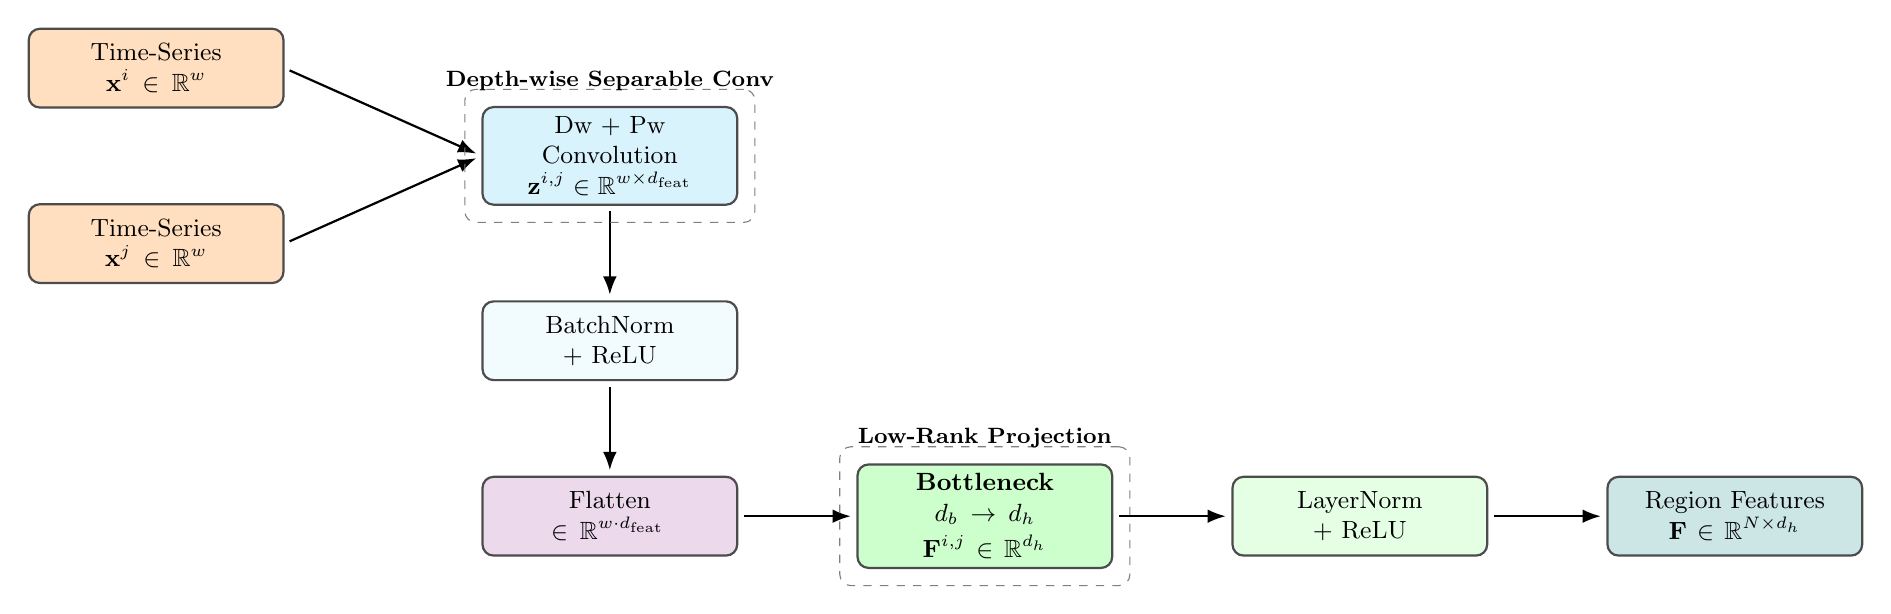
\begin{tikzpicture}[
    font=\small,
    >=Latex,
    block/.style={
        rectangle, draw=black!70, thick,
        rounded corners, align=center,
        minimum height=1cm,  % Increased height
        text width=3cm       % Increased width
    },
    arrow/.style={->, thick, shorten >=2pt, shorten <=2pt},
]
  %––– Inputs (split) –––––––––––––––––––––––––––––––––––––––
  \node (xi) [block, fill=orange!25] {Time‑Series\\$\mathbf{x}^i\!\in\!\mathbb{R}^{w}$};
  \node (xj) [block, fill=orange!25, below=1.2cm of xi] {Time‑Series\\$\mathbf{x}^j\!\in\!\mathbb{R}^{w}$};

  % Compute a point centred between xi and xj for tidy piping
  \path (xi.east) -- (xj.east) coordinate[midway] (midinput);

  %––– Pipeline nodes –––––––––––––––––––––––––––––––––––––––
  \node (sepconv) [block, fill=cyan!15,  right=2.5cm of midinput] {
      Dw + Pw\\Convolution\\
      $\mathbf{z}^{i,j}\!\in\!\mathbb{R}^{w\times d_{\text{feat}}}$};

  \node (bn)   [block, fill=cyan!5, below=1.2cm of sepconv] {BatchNorm\\+ ReLU};

  \node (flat) [block, fill=violet!15, below=1.2cm of bn] {Flatten\\$\!\in\!\mathbb{R}^{w\cdot d_{\text{feat}}}$};

  % Horizontal arrangement for the remaining nodes
  \node (proj) [block, fill=green!20, right=1.5cm of flat] {
      \textbf{Bottleneck}\\$d_b\!\to\! d_h$\\[2pt]
      $\mathbf{F}^{i,j}\!\in\!\mathbb{R}^{d_{h}}$};

  \node (ln) [block, fill=green!10, right=1.5cm of proj] {LayerNorm\\+ ReLU};

  \node (output) [block, fill=teal!20, right=1.5cm of ln] {Region Features\\$\mathbf{F}\!\in\!\mathbb{R}^{N\times d_{h}}$};

  %––– Arrows –––––––––––––––––––––––––––––––––––––––––––––––
  \draw[arrow] (xi.east) -- (sepconv.west);
  \draw[arrow] (xj.east) -- (sepconv.west);
  \draw[arrow] (sepconv.south) -- ++(0,-0.6) -- (bn.north);
  \draw[arrow] (bn.south) -- ++(0,-0.6) -- (flat.north);
  \draw[arrow] (flat.east) -- (proj.west);
  \draw[arrow] (proj.east) -- (ln.west);
  \draw[arrow] (ln.east) -- (output.west);

  %––– Grouping boxes –––––––––––––––––––––––––––––––––––––––
  \usetikzlibrary{fit}
  % \begin{scope}[on background layer] % Removed for IEEEtran compatibility
    \node[draw=black!50, dashed, rounded corners, inner sep=6pt,
          fit=(sepconv)] {};
    \node at (sepconv.north) [above=2pt, font=\footnotesize\bfseries] {Depth‑wise Separable Conv};

    \node[draw=black!50, dashed, rounded corners, inner sep=6pt,
          fit=(proj)] {};
    \node at (proj.north) [above=2pt, font=\footnotesize\bfseries] {Low‑Rank Projection};
  % \end{scope} % Removed for IEEEtran compatibility
\end{tikzpicture}%
}
\caption{Feature‑extraction pipeline. Independent regional time‑series $\mathbf{x}^i$ and $\mathbf{x}^j$ are processed in parallel by depth‑wise and point‑wise convolutions, normalised, flattened, passed through a bottleneck projection ($d_b\!\to\! d_h$), and normalised again to yield region‑level feature vectors $\mathbf F$.}
\label{fig:feature_extraction}
\end{figure*}

\subsection{Efficient Adaptive Graph Attention with Low-Rank Decomposition}

The second core component of our MSAGAT-Net architecture is the Adaptive Graph Attention Module (AGAM). Traditional approaches to spatial modelling often rely on fixed adjacency matrices based on geographical proximity or administrative boundaries, which do not capture the evolving nature of epidemic spread influenced by factors such as population mobility, healthcare referral patterns, and socioeconomic connections. Based on the principles of graph attention networks \cite{velickovic2017graph}, our AGAM adaptively learns the relationships between regions based on their feature representations, rather than being constrained by a predefined graph structure. This adaptive approach allows the model to discover and leverage spatial dependencies that may not be immediately apparent from geographical proximity alone, and to adjust these dependencies as the epidemic evolves.

A significant challenge in implementing graph attention mechanisms for large-scale epidemic or forecasting problems is computational complexity. Standard softmax-based attention mechanisms in graph neural networks (GNNs) typically incur quadratic $\mathcal{O}(N^2)$ complexity with respect to the number of nodes, making them prohibitively expensive for large graphs. Additionally, these methods often suffer from over-smoothing when modelling long-range dependencies, where node representations become increasingly similar after multiple message-passing iterations.

Recent advances in efficient attention mechanisms have shown that low-rank decomposition techniques can substantially reduce computational complexity whilst maintaining expressive power. Several influential works have explored this direction. Researchers such as \cite{puny2020global} propose a low-rank global attention (LRGA), an adaptive module that replaces the total attention of the dot product in GNN with a decomposed low-rank form. \cite{kong2023low} present the Global Representation Key (GRK) attention layer, where the attention scores of each node are calculated using a shared projection of the features of its neighbours. A learnt adaptive low-rank matrix captures the most salient structural information, mitigating over-smoothing and improving performance on graphs. While \cite{yang2023self} embeds an adaptive low-rank decomposition step in each propagation layer within each ego network to concentrate message passing on the most prominent low-dimensional subspaces. This lets the model adaptively focus on the most informative subspace per node, improving robustness without labels. These studies collectively demonstrate that low-rank factorisation offers an efficient, scalable and expressive alternative to full-rank attention in graph architectures, motivating the design of this module in our framework.

Motivated by these advances, AGAM employs a linearised attention mechanism that combines low-rank decomposition with a novel graph bias message passing mechanism. Rather than computing the full attention matrix between all pairs of regions (which incurs $\mathcal{O}(N^2)$ complexity for traditional softmax attention), we use a linearised formulation that reduces complexity to $\mathcal{O}(N)$ through fixed-rank bottleneck projections (bottleneck dimension $d_b = 8$), scaling linearly with the number of regions. Efficiency arises from (i) low-rank bottleneck projections for query, key, and value representations, and (ii) a linearised attention computation that avoids explicit construction of the $N\times N$ attention matrix whilst maintaining the capacity to learn complex spatial dependencies. A key innovation of our approach is the integration of a learnable graph bias directly into the forward computation through normalised low-rank message passing, rather than using it solely for regularisation as in prior work. This enables the model to leverage persistent spatial relationships during inference whilst maintaining linear complexity. The AGAM module comprises six components: (1) bottleneck projections for QKV, (2) multi-head attention with ELU-based linearisation, (3) normalisation for numerical stability, (4) learnable graph structure bias, (5) graph bias message passing for forward integration, and (6) attention regularisation to promote sparsity. 

\subsubsection{Bottleneck Projection}

Given the feature matrix $\mathbf{F} \in \mathbb{R}^{N \times d_{\text{hidden}}}$ from the feature extraction module, where $N$ is the number of regions and $d_{\text{hidden}}$ is the hidden dimension, we first project these features into query, key, and value representations through an efficient bottleneck projection:

\begin{equation}
\mathbf{Q}_{\text{low}}, \mathbf{K}_{\text{low}}, \mathbf{V}_{\text{low}} = \text{Split}(\text{Linear}_{\text{low}}(\mathbf{F}), 3)
\end{equation}

where $\text{Linear}_{\text{low}}: \mathbb{R}^{d_{\text{hidden}}} \rightarrow \mathbb{R}^{3 \times d_{\text{bottle}}}$ projects the features into a lower-dimensional space and $\text{Split}$ divides the output into three separate tensors of dimension $\mathbb{R}^{N \times d_{\text{bottle}}}$.

These low-dimensional projections are then expanded back to the full hidden dimension:

\begin{equation}
\mathbf{Q}, \mathbf{K}, \mathbf{V} = \text{Split}(\text{Linear}_{\text{high}}([\mathbf{Q}_{\text{low}}; \mathbf{K}_{\text{low}}; \mathbf{V}_{\text{low}}]), 3)
\end{equation}

where $\text{Linear}_{\text{high}}: \mathbb{R}^{3 \times d_{\text{bottle}}} \rightarrow \mathbb{R}^{3 \times d_{\text{hidden}}}$ and each of $\mathbf{Q}, \mathbf{K}, \mathbf{V} \in \mathbb{R}^{N \times d_{\text{hidden}}}$.

This bottleneck projection significantly reduces the parameter count from $\mathcal{O}(3 \times d_{\text{hidden}}^2)$ to $\mathcal{O}(3 \times d_{\text{hidden}} \times d_{\text{bottle}})$, where $d_{\text{bottle}} \ll d_{\text{hidden}}$.

\subsubsection{Multi-Head Attention Mechanism}

To enhance the model's capacity to capture different types of inter-regional relationships, we implement a multi-head attention mechanism where the hidden representations are split into $h$ heads, each with dimension $d_{\text{head}} = d_{\text{hidden}} / h$:

\begin{equation}
\mathbf{Q}^{(i)}, \mathbf{K}^{(i)}, \mathbf{V}^{(i)} \in \mathbb{R}^{N \times d_{\text{head}}}, \quad i \in \{1, 2, \ldots, h\}
\end{equation}

For efficient computation, we reshape these tensors to explicitly represent the multiple heads:

\begin{equation}
\mathbf{Q}_h = \text{Reshape}(\mathbf{Q}, [N, h, d_{\text{head}}])
\end{equation}
\begin{equation}
\mathbf{K}_h = \text{Reshape}(\mathbf{K}, [N, h, d_{\text{head}}])
\end{equation}
\begin{equation}
\mathbf{V}_h = \text{Reshape}(\mathbf{V}, [N, h, d_{\text{head}}])
\end{equation}

We then transpose the first two dimensions to facilitate batch-wise processing across attention heads:

\begin{equation}
\mathbf{Q}_h, \mathbf{K}_h, \mathbf{V}_h = \text{Transpose}(\mathbf{Q}_h, 0, 1), \text{Transpose}(\mathbf{K}_h, 0, 1), \text{Transpose}(\mathbf{V}_h, 0, 1)
\end{equation}

resulting in tensors of shape $[h, N, d_{\text{head}}]$.

A key innovation in our approach is the specific attention computation mechanism employed within each head. Rather than relying on standard scaled dot-product attention with softmax, we employ an enhanced mechanism with better numerical stability and more nuanced relationship modelling.

First, we apply the Exponential Linear Unit (ELU) activation function followed by adding a constant value of 1 to both query and key representations:

\begin{equation}
\hat{\mathbf{Q}}_h = \text{ELU}(\mathbf{Q}_h) + 1
\end{equation}
\begin{equation}
\hat{\mathbf{K}}_h = \text{ELU}(\mathbf{K}_h) + 1
\end{equation}

This transformation ensures that all attention inputs are positive, improving gradient stability during training whilst allowing for more flexible attention patterns than the standard dot-product attention.

Next, we compute the key-value product for each attention head:

\begin{equation}
\mathbf{KV}_h = \hat{\mathbf{K}}_h^T \mathbf{V}_h
\end{equation}

where $\mathbf{KV}_h \in \mathbb{R}^{h \times d_{\text{head}} \times d_{\text{head}}}$. This operation captures the relationships between keys and values, allowing the model to learn how to weight the features of different regions based on their similarity.

To ensure stable normalisation, we calculate a normalisation factor based on the sum of keys:

\begin{equation}
\mathbf{z} = \frac{1}{\hat{\mathbf{K}}_h \cdot \mathbf{1} + \epsilon}
\end{equation}

where $\mathbf{1}$ is a vector of ones and $\epsilon$ is a small constant ($10^{-8}$ in our implementation) to prevent division by zero. This operation ensures stable normalisation across the attention heads, allowing for effective learning of inter-regional relationships. 

The final attention output for each head is computed as:

\begin{equation}
\mathbf{O}_h = \hat{\mathbf{Q}}_h \mathbf{KV}_h \mathbf{z}
\end{equation}

where $\mathbf{O}_h \in \mathbb{R}^{h \times N \times d_{\text{head}}}$ represents the attended features across all heads.

\subsubsection{Learnable Graph Structure}

An important feature of our AGAM is the incorporation of a learnable graph structure bias. Unlike traditional graph attention networks that rely solely on node features for computing attention, we include a learnable bias term that captures persistent structural relationships between regions that may not be evident from the node features alone.

This bias is implemented as a low-rank decomposition for parameter efficiency:

\begin{equation}
\mathbf{B} = \mathbf{U} \mathbf{V}
\end{equation}

where $\mathbf{U} \in \mathbb{R}^{h \times N \times d_{\text{bias}}}$ and $\mathbf{V} \in \mathbb{R}^{h \times d_{\text{bias}} \times N}$ are learnable parameters and $d_{\text{bias}} \ll N$ is the bottleneck dimension of the bias term. This learnable bias $\mathbf{B} \in \mathbb{R}^{h \times N \times N}$ provides an innovative mechanism for the model to learn persistent spatial structures that complement data-driven attention patterns.

\subsubsection{Graph Bias Message Passing}

Rather than using the graph bias solely for regularisation, we integrate it directly into the forward computation through a normalised low-rank message passing operation. This approach maintains $\mathcal{O}(N)$ complexity by exploiting the low-rank factorisation $\mathbf{B} = \mathbf{U}\mathbf{V}$ to avoid materialising the full $N \times N$ bias matrix.

To ensure stable message passing with non-negative weights, we first apply a positivity transformation to the low-rank factors:

\begin{equation}
\hat{\mathbf{U}} = \text{ELU}(\mathbf{U}) + 1, \quad \hat{\mathbf{V}} = \text{ELU}(\mathbf{V}) + 1
\end{equation}

The graph bias message passing output is then computed as:

\begin{equation}
\mathbf{O}_{\text{bias}} = \frac{\hat{\mathbf{U}} (\hat{\mathbf{V}} \mathbf{V}_h)}{\hat{\mathbf{U}} (\hat{\mathbf{V}} \mathbf{1}) + \epsilon}
\end{equation}

where $\mathbf{V}_h$ represents the value representations, $\mathbf{1}$ is a vector of ones, and $\epsilon = 10^{-8}$ prevents division by zero. The numerator computes $\hat{\mathbf{U}} (\hat{\mathbf{V}} \mathbf{V}_h) \in \mathbb{R}^{h \times N \times d_{\text{head}}}$ through two sequential matrix multiplications, each with complexity $\mathcal{O}(N \cdot d_{\text{bias}} \cdot d_{\text{head}})$. The denominator provides row-wise normalisation analogous to the normalisation in standard attention mechanisms.

This message passing output is combined with the linear attention output:

\begin{equation}
\mathbf{O}_h = \mathbf{O}_{\text{linear}} + \text{Dropout}(\mathbf{O}_{\text{bias}})
\end{equation}

By integrating the learned graph structure directly into the forward pass, the model can leverage persistent spatial relationships during inference whilst maintaining the computational efficiency of linearised attention.

\subsubsection{Attention Regularisation}

To promote sparse and interpretable spatial relationships, we apply L1 regularisation to the graph structure bias:

\begin{equation}
\mathcal{L}_{\text{attn}} = \lambda \|\mathbf{B}\|_1
\end{equation}

where $\lambda$ is the learnable regularisation weight. This regularisation encourages the model to learn sparse, interpretable spatial dependency patterns in the graph bias whilst maintaining the computational efficiency of linearised attention. The value of $\lambda$ is initialised to $10^{-5}$ and adapted during training through gradient descent in log-domain (ensuring positivity), allowing the model to automatically balance forecast accuracy with attention sparsity.

After computing the attended values for each head, we combine them and project back to the original feature dimension:

\begin{equation}
\mathbf{O} = \text{Reshape}(\text{Transpose}(\mathbf{O}_h, 0, 1), [N, d_{\text{hidden}}])
\end{equation}

Similarly to the input projection, we employ a low-rank output projection for efficiency:

\begin{equation}
\mathbf{O}_{\text{low}} = \text{Linear}_{\text{out\_low}}(\mathbf{O})
\end{equation}

\begin{equation}
\mathbf{O}_{\text{final}} = \text{Linear}_{\text{out\_high}}(\mathbf{O}_{\text{low}})
\end{equation}

where $\mathbf{O}_{\text{low}} \in \mathbb{R}^{N \times d_{\text{bottle}}}$ and $\mathbf{O}_{\text{final}} \in \mathbb{R}^{N \times d_{\text{hidden}}}$.

The output of AGAM, $\mathbf{O}_{\text{final}}$, represents the features of the region after incorporating spatial dependencies. This output, along with the attention regularisation loss $\mathcal{L}_{\text{attn}}$, is passed to the subsequent MTFM for further processing.

For the AGAM module, we set the number of attention heads to $h=4$ and the bottleneck dimension to $d_{\text{bottle}}=8$. These values were determined through preliminary experiments to provide an optimal balance between capturing diverse spatial dependency patterns and the maintenance of computational efficiency through low-rank decomposition. The attention regularisation weight $\lambda$ is set to $10^{-5}$, which was empirically found to promote sparse, interpretable attention patterns without overly constraining the model's capacity to learn complex spatial relationships. This configuration allows AGAM to model dynamic spatial dependencies efficiently whilst avoiding the computational overhead of full-rank attention mechanisms. Figure~\ref{fig:agam_module} presents the data flow through the AGAM module. 

% The AGAM module introduces several key advantages for epidemic forecasting:

% \begin{enumerate}
%     \item \textbf{Adaptive spatial modelling}: By learning attention weights dynamically, the model can adapt to changing spatial dependencies over time, crucial for capturing evolving epidemic spread patterns.
    
%     \item \textbf{Computational efficiency}: The low-rank projections and decompositions significantly reduce the parameter count and computational complexity, enabling the model to scale to large numbers of regions.
    
%     \item \textbf{Interpretability}: The learnt attention patterns can provide valuable insights into region-to-region influence, potentially helping epidemiologists identify key transmission pathways.
    
%     \item \textbf{Integration of prior knowledge}: The learnable graph structure bias allows the model to incorporate domain knowledge about regional connections whilst still adapting to data-driven patterns.
% \end{enumerate}

% Through these innovations, the AGAM effectively captures the complex spatial dependencies inherent in epidemic data, providing a solid foundation for the subsequent temporal modelling steps in our architecture.


\begin{figure*}[!htbp]
\centering
%–— 1. We still fix the width to \linewidth; the height now shrinks naturally –—
\resizebox{\linewidth}{!}{%
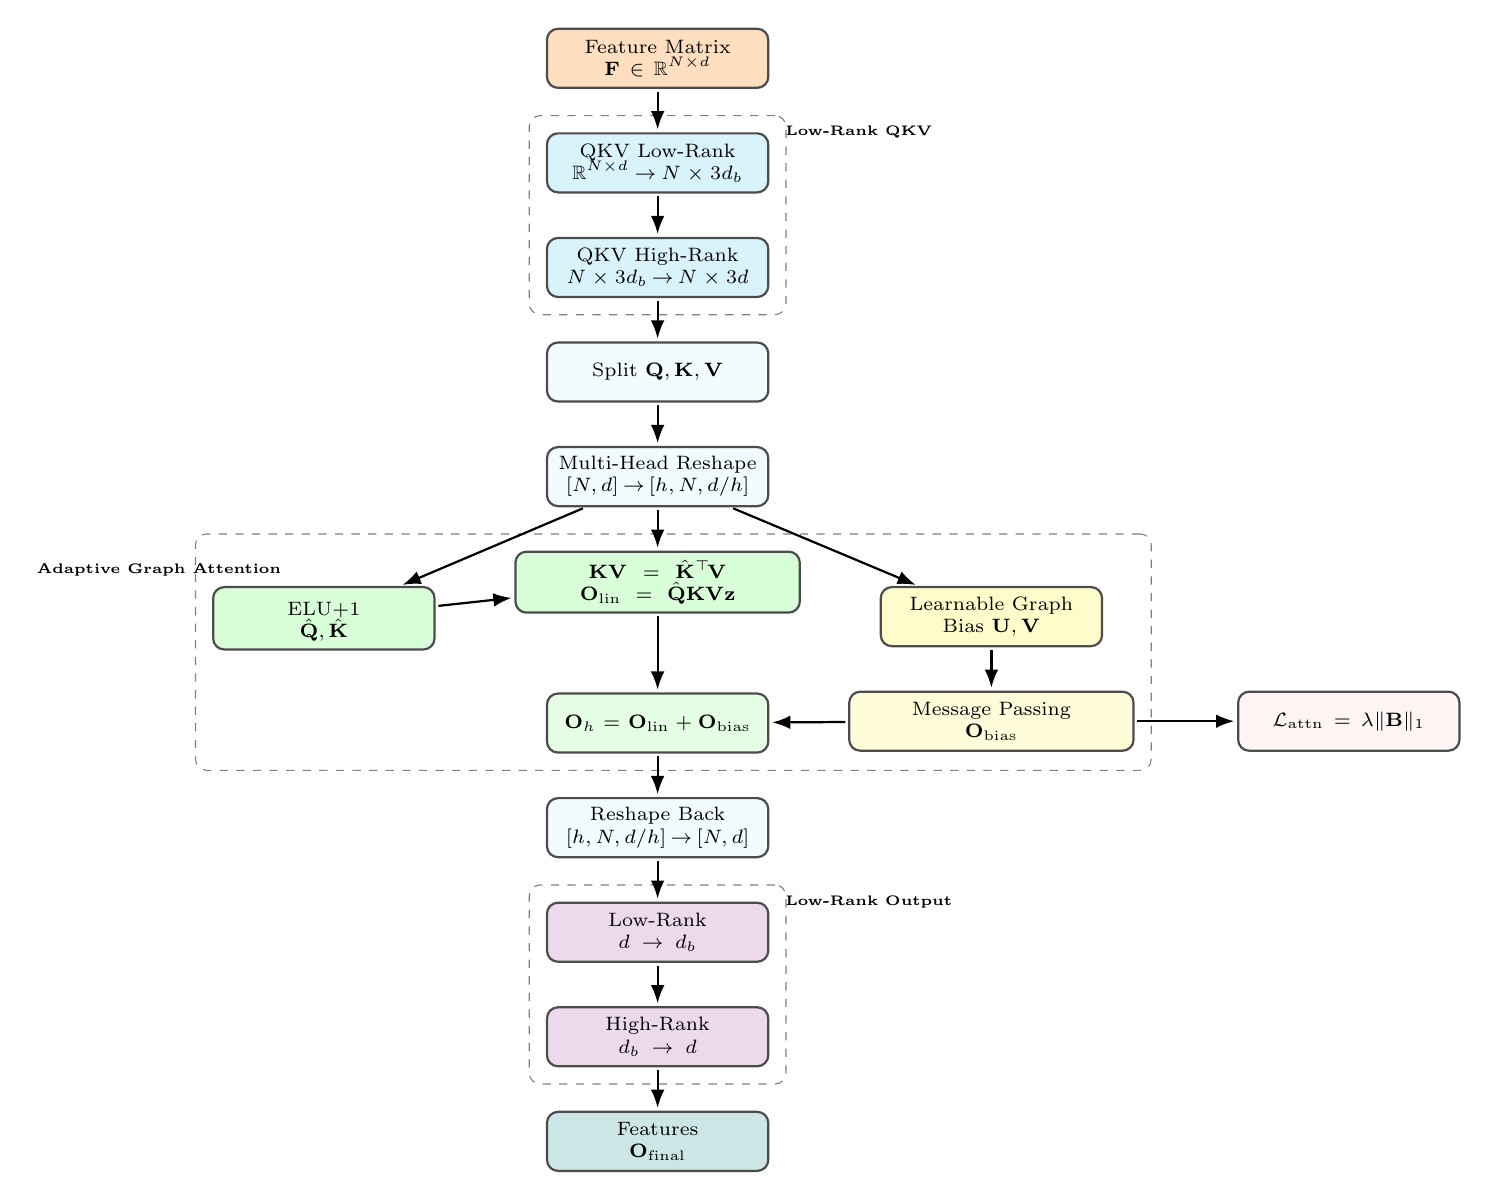
\begin{tikzpicture}[
    %–––– GLOBAL STYLE TWEAKS ––––
    font=\scriptsize,                                % smaller text
    >=Latex,
    node distance = 0.55cm and 1.6cm,                % default vert / horiz gap
    block/.style = {rectangle, draw=black!70, thick,
                    rounded corners, align=center,
                    minimum height=0.75cm,           % lower boxes
                    text width=2.6cm,                % narrower boxes
                    inner sep=3pt},                  % tighter padding
    wideblock/.style = {block, text width=3.4cm},    % a bit wider
    arrow/.style = {->, thick, shorten >=1pt, shorten <=1pt},
]
%–––– MAIN FLOW ––––
\node (input)      [block, fill=orange!25] {Feature Matrix\\$\mathbf{F}\!\in\!\mathbb{R}^{N\times d}$};

\node (qkv_low)    [block,  fill=cyan!15,  below=of input]          {QKV Low‑Rank\\$\mathbb{R}^{N\times d}\!\to\! N\times3d_b$};

\node (qkv_high)   [block,  fill=cyan!15,  below=of qkv_low]        {QKV High‑Rank\\$N\times3d_b\!\to\! N\times3d$};

\node (split)      [block,  fill=cyan!5,   below=of qkv_high]       {Split $\mathbf Q,\mathbf K,\mathbf V$};

\node (reshape)    [block,  fill=cyan!5,   below=of split]          {Multi‑Head Reshape\\$[N,d]\!\to\![h,N,d/h]$};

%–––– PARALLEL BRANCH (three nodes at same depth) ––––
\node (qk_proc)    [block,  fill=green!15, below left=1.0cm and 1.4cm of reshape] {\rule{0pt}{0.9em}ELU$+1$\\$\hat{\mathbf Q},\hat{\mathbf K}$};

\node (graph_bias) [block,  fill=yellow!20, below right=1.0cm and 1.4cm of reshape] {Learnable Graph\\Bias $\mathbf{U}, \mathbf{V}$};

\node (attn_comp)  [wideblock, fill=green!15, below=of reshape]     {$\mathbf{KV}=\hat{\mathbf K}^\top\!\mathbf V$\\
                                                                     $\mathbf O_{\text{lin}}=\hat{\mathbf Q}\mathbf{KV}\mathbf z$};

%–––– MESSAGE PASSING / REG ––––
\node (msg_pass)[wideblock, fill=yellow!15, below=of graph_bias]  {Message Passing\\$\mathbf O_{\text{bias}}$};

\node (attn_reg)   [block,      fill=pink!15,  right=1.3cm of msg_pass] {$\mathcal L_{\text{attn}}=\lambda\|\mathbf B\|_1$};

\node (combine)    [block,  fill=green!10, below=1.0cm of attn_comp]  {$\mathbf O_h = \mathbf O_{\text{lin}} + \mathbf O_{\text{bias}}$};

%–––– OUTPUT PATH ––––
\node (reshape_out) [block, fill=cyan!5,   below=of combine] {Reshape Back\\$[h,N,d/h]\!\to\![N,d]$};

\node (out_low)     [block, fill=violet!15, below=of reshape_out]   {Low‑Rank\\$d\!\to\! d_b$};

\node (out_high)    [block, fill=violet!15, below=of out_low]       {High‑Rank\\$d_b\!\to\! d$};

\node (output)      [block, fill=teal!20,   below=of out_high]      {Features\\$\mathbf O_{\text{final}}$};

%–––– ARROWS ––––
\foreach \a/\b in {
  input/qkv_low, qkv_low/qkv_high, qkv_high/split, split/reshape,
  reshape/qk_proc, reshape/attn_comp, reshape/graph_bias,
  qk_proc/attn_comp, graph_bias/msg_pass,
  msg_pass/attn_reg, msg_pass/combine, attn_comp/combine,
  combine/reshape_out, reshape_out/out_low, out_low/out_high, out_high/output}
  \draw[arrow] (\a) -- (\b);

%–––– GROUP BOXES (dashed) ––––
\usetikzlibrary{fit}
\begin{scope}[on background layer]
  \node [draw=black!50, dashed, rounded corners, inner sep=6pt,
         fit=(qkv_low)(qkv_high)] {};
  \node at (qkv_low.north) [above=1pt, right=0pt and 1.5cm, font=\tiny\bfseries] {Low-Rank QKV};

  \node [draw=black!50, dashed, rounded corners, inner sep=6pt,
         fit=(qk_proc)(attn_comp)(graph_bias)(msg_pass)(combine)] {};
  \node at (qk_proc.north west) [above left=0pt and -1.0cm, font=\tiny\bfseries] {Adaptive Graph Attention};

  \node [draw=black!50, dashed, rounded corners, inner sep=6pt,
         fit=(out_low)(out_high)] {};
  \node at (out_low.north) [above=1pt, right=0pt and 1.5cm, font=\tiny\bfseries] {Low-Rank Output};
\end{scope}
\end{tikzpicture}}%
% \caption{Flow of data and structure in the AGAM module.}
\caption{Data flow in the AGAM module. Input features undergo low-rank QKV projections, followed by linearised attention computation. The learnable graph bias is integrated via normalised message passing, and L1 regularisation promotes sparse spatial patterns.}
\label{fig:agam_module}
\end{figure*}

Figure \ref{fig:agam_module} illustrates the flow of data through the AGAM module. The input feature matrix $\mathbf{F}$ is processed through low-rank projections to obtain query, key, and value representations. These representations are reshaped for multi-head attention computation, where the linearised attention mechanism with ELU+1 kernel trick is applied. The learnable graph structure bias is integrated into the forward pass through normalised low-rank message passing, combining with the linear attention output. L1 regularisation on the graph bias promotes sparse, interpretable spatial dependency patterns. Finally, the output features are obtained through low-rank output projections, ready for further processing in MTFM.

\subsection{Multi-Scale Temporal Feature Module}

The third major component of our MSAGAT-Net architecture is the Multi-Scale Temporal Feature Module (MTFM), which addresses a fundamental challenge in epidemic forecasting: modelling temporal dependencies across multiple time scales. Epidemics exhibit complex temporal dynamics that span various scales, including short-term fluctuations (e.g., reporting delays or weekend effects), medium-term patterns (e.g., incubation or transmission cycles), and long-term trends (e.g., seasonal variations or behavioural changes) \cite{Stone2007Seasonal, Panja2022Epicasting, Qiu2024MSGNN}. Accurate forecasting therefore requires models capable of effectively capturing these multi-scale temporal dynamics.

Deng et al. \cite{dengColaGNNCrosslocationAttention2020a} introduce the idea of multi-scale dilated convolutional with the same filter and stride sides but different dilation rates, which Xie et al. \cite{xie2022epignn} improved by making use of the multi-scale convolution to capture features. Building on this, the MTFM employs parallel dilated convolutional layers to efficiently capture temporal dependencies across multiple scales using the output from the AGAM. This approach enables the model to maintain an awareness of both immediate and distant temporal relationships whilst controlling parameter count and computational complexity.


\subsubsection{Dilated Convolutions for Multi-scale Processing}

The core of our MTFM is a set of parallel convolutional branches operating at different dilation rates. For a given input feature tensor $\mathbf{G} \in \mathbb{R}^{B \times N \times d_{\text{hidden}}}$ (where $B$ is the batch size, $N$ is the number of regions, and $d_{\text{hidden}}$ is the hidden dimension), we first transpose the tensor to prepare for 1D convolutions along the temporal dimension:

\begin{equation}
\mathbf{G}_{\text{conv}} = \text{Transpose}(\mathbf{G}, 1, 2)
\end{equation}

resulting in a tensor of shape $[B, d_{\text{hidden}}, N]$. We then process this tensor through $S$ parallel branches, each consisting of a dilated convolutional layer with a specific dilation rate, followed by batch normalisation, ReLU activation and dropout:

\begin{equation}
\mathbf{H}^{(i)} = \text{Dropout}(\text{ReLU}(\text{BatchNorm}(\text{Conv1D}(\mathbf{G}_{\text{conv}}; k, d^{(i)}))))
\end{equation}

where $i \in \{1, 2, \ldots, S\}$ indexes the scale, $k$ is the kernel size (set to 3 by default), and $d^{(i)} = 2^{i-1}$ is the dilation rate for the scale $i$. Each branch produces an output tensor $\mathbf{H}^{(i)} \in \mathbb{R}^{B \times d_{\text{hidden}} \times N}$.

The increasing dilation rates create an exponentially expanding receptive field across the branches. For a dilated convolution with kernel size $k$ and dilation rate $d$, the receptive field is given by:

\begin{equation}
RF = (k - 1) \times d + 1
\end{equation}

With $k=3$, this yields: Scale 1 ($d^{(1)} = 1$) captures immediate temporal dependencies with a receptive field of $(3-1) \times 1 + 1 = 3$ time steps. Scale 2 ($d^{(2)} = 2$) captures medium-range dependencies with a receptive field of $(3-1) \times 2 + 1 = 5$ time steps. Scale 3 ($d^{(3)} = 4$) captures longer-range dependencies with a receptive field of $(3-1) \times 4 + 1 = 9$ time steps. These three scales provide sufficient coverage for typical epidemic dynamics within a 20-day lookback window, whilst a fourth scale ($d=8$, RF=17) would approach the window boundary with diminishing returns.

This multi-scale approach allows the model to efficiently capture a wide range of temporal dependencies without requiring deep sequential processing, which is particularly advantageous for epidemic time-series that often exhibit both rapid changes and gradual trends.

\subsubsection{Adaptive Scale Fusion}

Rather than simply concatenating or averaging the outputs from different scales, we implement an adaptive fusion mechanism that allows the model to learn the relative importance of each temporal scale. This is achieved through learnable fusion weights:

\begin{equation}
\boldsymbol{\alpha} = \text{softmax}(\mathbf{w})
\end{equation}

where $\mathbf{w} \in \mathbb{R}^S$ is a learnable parameter vector and $\boldsymbol{\alpha} \in \mathbb{R}^S$ represents the normalised importance weights for each scale.

The multi-scale features are then fused using these weights:

\begin{equation}
\mathbf{H}_{\text{fused}} = \sum_{i=1}^{S} \alpha_i \mathbf{H}^{(i)}
\end{equation}

where $\mathbf{H}_{\text{fused}} \in \mathbb{R}^{B \times d_{\text{hidden}} \times N}$ is the scale-fused feature representation.

\begin{figure*}[!t]
\centering
\includegraphics[width=0.7\textwidth]{figs/mtfm_diagram.pdf}
% \caption{Flow of data in the MTFM architecture.}
\caption{Data flow in the MTFM module. Spatial features from AGAM are processed through three parallel dilated convolutional branches (dilation rates 1, 2, 4), adaptively fused using learnable weights, and combined with residual connections.}
\label{fig:mtfm_module}
\end{figure*}

\subsubsection{Bottleneck Projection and Residual Connection}

To enhance training stability and allow for more effective feature transformation, we apply a low-rank bottleneck projection to the fused features:

\begin{equation}
\mathbf{H}_{\text{low}} = \text{Linear}_{\text{fusion\_low}}(\text{Transpose}(\mathbf{H}_{\text{fused}}, 1, 2))
\end{equation}

\begin{equation}
\mathbf{H}_{\text{proj}} = \text{Linear}_{\text{fusion\_high}}(\mathbf{H}_{\text{low}})
\end{equation}

where $\mathbf{H}_{\text{low}} \in \mathbb{R}^{B \times N \times d_{\text{bottle}}}$ is the bottleneck representation with dimension $d_{\text{bottle}} \ll d_{\text{hidden}}$, and $\mathbf{H}_{\text{proj}} \in \mathbb{R}^{B \times N \times d_{\text{hidden}}}$ is the projected representation.

We then apply layer normalisation and a residual connection to facilitate gradient flow during training:

\begin{equation}
\mathbf{H}_{\text{final}} = \text{LayerNorm}(\text{Transpose}(\mathbf{H}_{\text{fused}}, 1, 2) + \mathbf{H}_{\text{proj}})
\end{equation}

where $\mathbf{H}_{\text{final}} \in \mathbb{R}^{B \times N \times d_{\text{hidden}}}$ is the final output of the MTFM.

For the MTFM module, we set the number of temporal scales to $S=3$ with exponentially increasing dilation rates of $\{1, 2, 4\}$ and a convolutional kernel size of $k=3$. This configuration was empirically determined to provide optimal coverage: with a typical lookback window of $w=20$ time steps, the three scales capture receptive fields of 3, 5, and 9 time steps respectively, spanning immediate to weekly-scale patterns. A fourth scale ($d=8$) would yield a receptive field of 17 steps, approaching the window boundary with diminishing returns and increased risk of overfitting. Our ablation studies (Section~\ref{sec:ablation}) corroborate this design choice, showing that additional temporal complexity can occasionally degrade performance on epidemic data. The hidden dimension $d_{\text{hidden}}$ is preserved throughout the module to maintain information capacity, whilst the bottleneck dimension within each scale is set to $d_{\text{bottle}} = d_{\text{hidden}}/4$ to reduce parameters in the projection layers. To mitigate overfitting on the noisy and often irregular epidemic time-series, we apply dropout with probability 0.25 after each convolutional layer and ReLU activation to regularise the model. Figure~\ref{fig:mtfm_module} presents a detailed representation of this module's architecture. 


\subsection{Progressive Multi-Horizon Forecast Refinement}

The final component of our MSAGAT-Net architecture is the Progressive Prediction Refinement Module (PPRM), which generates accurate forecasts across multiple future time steps. Multi-horizon forecasting presents a significant challenge in epidemiological prediction: whilst the preceding modules extract spatiotemporal features, converting these features into reliable forecasts requires addressing how forecast errors can compound over extended horizons.

The existing literature demonstrates that forecast errors accumulate with increasing forecast horizons \cite{BENTAIEB20127067, chandra2021evaluation}, making direct multistep prediction particularly challenging. The PPRM addresses this by incorporating an adaptive refinement mechanism that balances model-based forecasts with trend-based extrapolations. This design draws on concepts from adaptive gating mechanisms in recurrent neural networks \cite{hochreiter1997long} and is motivated by the observation that the recent epidemic trajectory provides valuable information for near-term forecasting.

\subsubsection{Low-Rank Forecast Projection}

Given the spatiotemporal feature tensor $\mathbf{H}_{\text{final}} \in \mathbb{R}^{B \times N \times d_{\text{hidden}}}$ from the Multi-Scale Temporal Feature Module, where $B$ is the batch size, $N$ is the number of regions, and $d_{\text{hidden}}$ is the hidden dimension, we first apply a bottleneck projection to distil the most forecast-relevant information:

\begin{equation}
\mathbf{P}_{\text{low}} = \text{Linear}_{\text{pred\_low}}(\mathbf{H}_{\text{final}})
\end{equation}

where $\mathbf{P}_{\text{low}} \in \mathbb{R}^{B \times N \times d_{\text{bottle}}}$ is the bottleneck representation with dimension $d_{\text{bottle}} \ll d_{\text{hidden}}$. This projection reduces dimensionality before the final forecast layer, reducing the parameter count whilst encouraging compact feature representations.

We then apply layer normalisation, ReLU activation, and dropout to the bottleneck representation:

\begin{equation}
\mathbf{P}_{\text{mid}} = \text{Dropout}(\text{ReLU}(\text{LayerNorm}(\mathbf{P}_{\text{low}})))
\end{equation}

This intermediate processing enhances training stability and introduces non-linearity necessary for modelling complex forecast patterns.

\subsubsection{Horizon-Specific Prediction}

From the processed bottleneck representation, we generate initial predictions for all forecast horizons using a linear projection:

\begin{equation}
\mathbf{P}_{\text{initial}} = \text{Linear}_{\text{pred\_high}}(\mathbf{P}_{\text{mid}})
\end{equation}

where $\mathbf{P}_{\text{initial}} \in \mathbb{R}^{B \times N \times h}$ represents the raw model forecasts for each region across all forecast horizons $h$.

To improve multi-horizon forecasting stability, we incorporate an adaptive refinement mechanism that combines these model-based forecasts with trend-based extrapolations from recent observations.

\subsubsection{Adaptive Refinement Mechanism}

The PPRM incorporates an adaptive refinement gate that balances model-based forecasts with trend-based extrapolations conditioned on the most recent observations.

We first compute an adaptive gate based on the spatiotemporal features:

\begin{equation}
\mathbf{G} = \sigma(\text{Linear}_{\text{gate\_high}}(\text{ReLU}(\text{Linear}_{\text{gate\_low}}(\mathbf{H}_{\text{final}}))))
\end{equation}

where $\mathbf{G} \in \mathbb{R}^{B \times N \times h}$ represents gate values between 0 and 1 for each region and forecast horizon, and $\sigma$ denotes the sigmoid activation function.

Currently, we use the most recent observation $\mathbf{x}_{\text{last}} \in \mathbb{R}^{B \times N}$ to generate a trend-based forecast using an exponential decay projection:

\begin{equation}
\mathbf{T} = \mathbf{x}_{\text{last}} \odot \exp(-\gamma \cdot \mathbf{d})
\end{equation}

where $\mathbf{x}_{\text{last}}$ is expanded to the shape $[B, N, h]$, $\mathbf{d} \in \mathbb{R}^h$ is a vector of increasing horizon indices $[1, 2, \ldots, h]$, $\gamma$ is a decay factor (set to 0.1 in our implementation), and $\odot$ represents element-wise multiplication.

This exponential decay formulation is inspired by epidemiological models that exhibit exponential growth or decay patterns, providing a simple yet effective baseline that captures the natural progression tendencies of epidemic time-series.

The final predictions are then computed as a weighted combination of the model-based predictions and the trend-based projections:

\begin{equation}
\mathbf{P}_{\text{final}} = \mathbf{G} \odot \mathbf{P}_{\text{initial}} + (1 - \mathbf{G}) \odot \mathbf{T}
\end{equation}

where $\mathbf{P}_{\text{final}} \in \mathbb{R}^{B \times N \times h}$ represents the refined forecasts for each region across all forecast horizons.

For the PPRM module, we set the bottleneck dimension at $d_{\text{bottle}}=8$ to maintain parameter efficiency while preserving sufficient capacity for the gating and refinement operations. The forecast horizon length $h$ is configurable based on task requirements; In our experiments, we primarily evaluate horizons of $h \in \{3, 5, 7, 10, 14, 15\}$ days, although the architecture supports arbitrary horizon lengths. The exponential decay factor $\gamma$ in the trend projection is set to 0.1, providing a moderate decay rate that was selected through empirical analysis of epidemic progression curves across our datasets and can be adjusted to match specific epidemic characteristics. We apply a dropout rate of 0.25 throughout the forecasting pathway to prevent overfitting, particularly critical for these final layers that directly generate model outputs. This dropout rate was determined through preliminary hyperparameter tuning to effectively regularise the model against the noisy and often irregular patterns characteristic of real-world epidemic surveillance data.


\begin{figure*}[!htbp]
\centering
% ~0.55·textheight; width adapts automatically
\resizebox{!}{0.55\textheight}{%
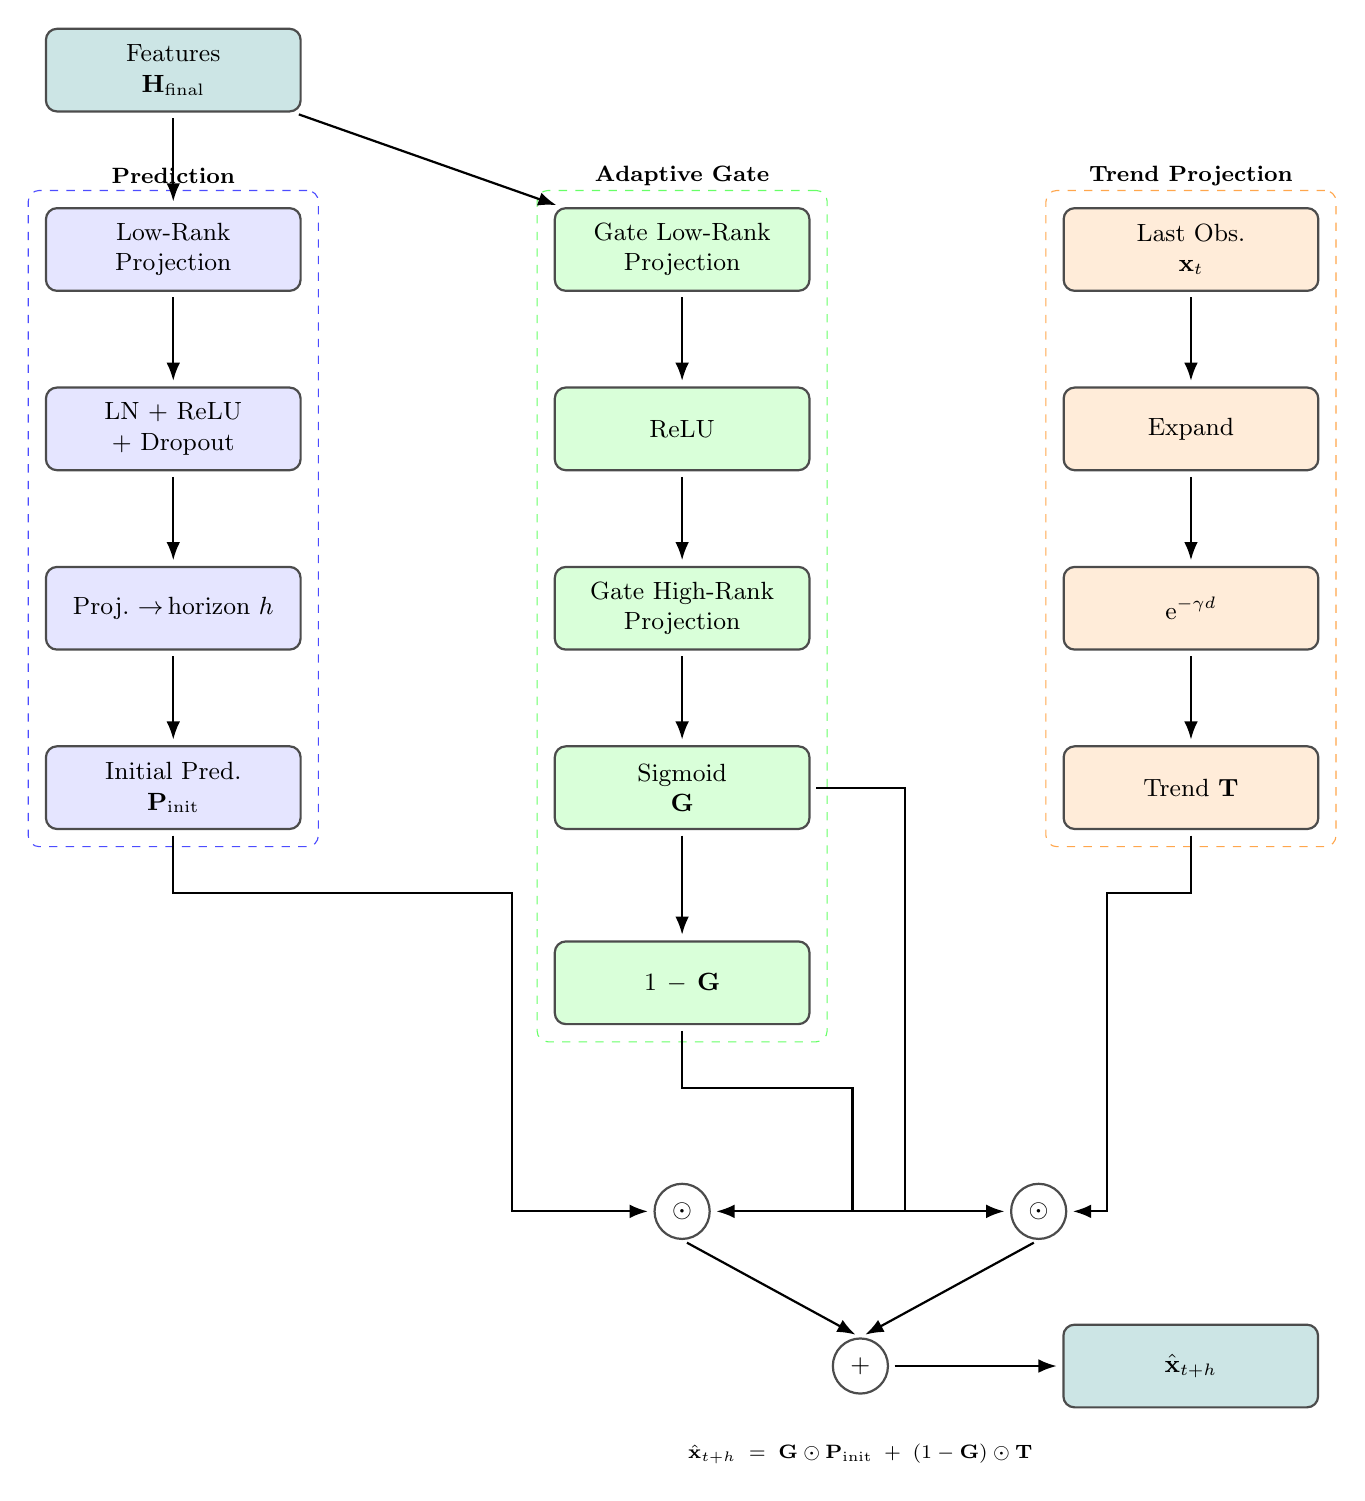
\begin{tikzpicture}[
    font=\small,
    >=Latex,
    node distance = 1.2cm and 1.8cm,
    block/.style={rectangle, draw=black!70, thick,
                  rounded corners, align=center,
                  minimum height=1.05cm, text width=3.0cm},
    pred/.style ={block, fill=blue!10},
    gate/.style ={block, fill=green!15},
    trend/.style={block, fill=orange!15},
    io/.style   ={block, fill=teal!20},
    op/.style   ={circle, draw=black!70, thick,
                  minimum size=0.7cm, inner sep=0pt},
    arrow/.style={->, thick, shorten >=2pt, shorten <=2pt}
]

%–––– INPUT –––––––––––––––––––––––––––––––––––––––––
\node (input) [io] {Features\\$\mathbf H_{\text{final}}$};

%–––– PREDICTION PATH ––––––––––––––––––––––––––––––
\node (plow)  [pred, below=of input]        {Low‑Rank\\Projection};
\node (pmid)  [pred, below=of plow]         {LN + ReLU + Dropout};
\node (phigh) [pred, below=of pmid]         {Proj. $\!\to\!$ horizon $h$};
\node (pinit) [pred, below=of phigh]        {Initial Pred.\\$\mathbf P_{\text{init}}$};

\foreach \a/\b in {input/plow, plow/pmid, pmid/phigh, phigh/pinit}
  \draw[arrow] (\a) -- (\b);

%–––– GATE PATH ––––––––––––––––––––––––––––––––––––
\node (glow)   [gate, right=3.2cm of plow]  {Gate Low‑Rank\\Projection};
\node (grelu)  [gate, below=of glow]        {ReLU};
\node (ghigh)  [gate, below=of grelu]       {Gate High‑Rank\\Projection};
\node (gsig)   [gate, below=of ghigh]       {Sigmoid\\$\mathbf G$};
\node (ginv)   [gate, below=1.4cm of gsig]  {$1-\mathbf G$};

\foreach \a/\b in {input/glow, glow/grelu, grelu/ghigh, ghigh/gsig, gsig/ginv}
  \draw[arrow] (\a) -- (\b);

%–––– TREND PATH –––––––––––––––––––––––––––––––––––
\node (last)   [trend, right=3.2cm of glow] {Last Obs.\\$\mathbf x_t$};
\node (expand) [trend, below=of last]       {Expand};
\node (decay)  [trend, below=of expand]     {$\mathrm e^{-\gamma d}$};
\node (trend)  [trend, below=of decay]      {Trend $\mathbf T$};

\foreach \a/\b in {last/expand, expand/decay, decay/trend}
  \draw[arrow] (\a) -- (\b);

% FUSION OPS (now lower)
% Products placed well below group boxes
\node (mul1) [op, below=2.0cm of ginv] {$\odot$};
\node (mul2) [op, right=3.8cm of mul1] {$\odot$};

% Sum centred beneath the products
\node (add)  [op, below=1.6cm of $(mul1)!0.5!(mul2)$] {$+$};

\node (output) [io, right=2.2cm of add] {$\hat{\mathbf x}_{t+h}$};

% Arrows from paths to products (entering from sides)
\draw[arrow] (pinit.south) -- ++ (0,-0.8) -| ($(mul1.west)+(-1.8,0)$) -- (mul1.west);
\draw[arrow] (gsig.east) -- ++ (1.2,0) |- (mul1.east);

\draw[arrow] (trend.south) -- ++ (0,-0.8) -| ($(mul2.east)+(0.5,0)$) -- (mul2.east);
\draw[arrow] (ginv.south) -- ++ (0,-0.8) -| ($(mul2.west)+(-2.0,0)$) -- (mul2.west);

% Products to sum, sum to output - direct connections are fine
\draw[arrow] (mul1.south) -- ($(mul1.south)!0.5!(add.north)$) -- (add.north);
\draw[arrow] (mul2.south) -- ($(mul2.south)!0.5!(add.north)$) -- (add.north);
\draw[arrow] (add.east) -- (output.west);

% EQUATION
\node (eq) [below=0.5cm of add, font=\scriptsize, align=center]
{$\displaystyle \hat{\mathbf x}_{t+h}\;=\;
        \mathbf G \odot \mathbf P_{\text{init}}
        \;+\;
        (1-\mathbf G) \odot \mathbf T$};

% GROUP BOXES
\usetikzlibrary{fit}
\begin{scope}[on background layer]
  \node[draw=blue!70,  dashed, rounded corners, inner sep=6pt,
        fit=(plow)(pmid)(phigh)(pinit)] {};
  \node at ($(plow.north)+(0,0.4)$) [font=\footnotesize\bfseries] {Prediction};

  \node[draw=green!60, dashed, rounded corners, inner sep=6pt,
        fit=(glow)(grelu)(ghigh)(gsig)(ginv)] {};
  \node at ($(glow.north)+(0,0.4)$) [font=\footnotesize\bfseries] {Adaptive Gate};

  \node[draw=orange!70, dashed, rounded corners, inner sep=6pt,
        fit=(last)(expand)(decay)(trend)] {};
  \node at ($(last.north)+(0,0.4)$) [font=\footnotesize\bfseries] {Trend Projection};
\end{scope}
\end{tikzpicture}}%
% \caption{The flow of data in the PPRM architecture}
\caption{Data flow in the PPRM module. Features are projected through a low-rank bottleneck to generate initial predictions. An adaptive gate learns to balance these model-based forecasts with exponential trend extrapolations based on recent observations.}
\label{fig:pprm_module}
\end{figure*}

Figure~\ref{fig:pprm_module} illustrates the flow of data through the PPRM module. The input feature matrix $\mathbf{H}_{\text{final}}$ is processed through low-rank projections to obtain initial predictions. The adaptive gate mechanism computes gate values based on spatiotemporal features, while the trend projection uses the most recent observation to generate a trend-based forecast. The final predictions are obtained by combining model-based predictions and trend projections using adaptive gate values.


\section{Experimental Setup}
\label{sec:experiments}

This section presents a comprehensive evaluation of our proposed MSAGAT-Net model across multiple epidemic datasets with varying characteristics. We compare MSAGAT-Net against strong baseline models to assess its effectiveness in capturing complex spatiotemporal dynamics and generating accurate multi-horizon forecasts. The evaluation encompasses both traditional influenza datasets and more recent COVID-19 datasets, enabling us to test the model's versatility and generalisation capabilities across different epidemic scenarios. We evaluated the models using multiple metrics, including root mean square error (RMSE), Pearson correlation coefficient (PCC), mean absolute error (MAE), and coefficient of determination (R²), to provide a complete performance assessment.

\subsection{Computing Environment}
\label{sec:experimental_setup}

All experiments were conducted on the same high performance computing (HPC) cluster equipped with NVIDIA RTX 8000 GPUs to ensure consistent hardware conditions in all model evaluations. This controlled environment allows for a fair comparison between different approaches and eliminates potential variations due to hardware differences.

\subsection{Datasets}
\label{sec:datasets}

To comprehensively evaluate the performance and generalisability of our proposed MSAGAT-Net framework, we performed experiments on several real-world epidemic datasets spanning various geographical regions, time periods, and disease types. This approach enables a thorough assessment of the model's versatility and robustness across varying spatio-temporal characteristics and epidemic scenarios.

Our experimental evaluation encompasses seven distinct datasets, each offering unique challenges and characteristics for epidemic forecasting. These datasets represent different geographical scales (from local authorities to national regions), temporal resolutions (daily and weekly measurements), and disease contexts (seasonal influenza and COVID-19). Table~\ref{tab:datasets} provides a statistical overview of these datasets, summarising their key characteristics and numerical properties.

\begin{table}[!htbp]
\centering
\caption{Overview of the epidemic datasets used in our experimental evaluation. ``Granularity'' indicates the temporal resolution of the epidemic data, whilst ``Size'' represents the product of the number of locations and the number of time steps.}
\label{tab:datasets}
\begin{tabular}{lccccc}
\hline
\textbf{Dataset} & \textbf{Size} & \textbf{Min} & \textbf{Max} & \textbf{Mean} & \textbf{Granularity} \\
\hline
Japan-Prefecture & $348 \times 47$ & 0 & 26,635 & 655 & Weekly \\
US-Region & $785 \times 10$ & 0 & 16,526 & 1,009 & Weekly \\
US-State & $360 \times 49$ & 0 & 9,716 & 223 & Weekly \\
Spain-COVID & $122 \times 35$ & 0 & 4,623 & 38 & Daily \\
Australia-COVID & $556 \times 8$ & 0 & 9,987 & 539 & Daily \\
LTLA-COVID & $839 \times 372$ & 0 & 4,170 & 85 & Daily \\
NHS-ICUBeds & $895 \times 7$ & 0 & 1,215 & 102 & Daily \\
\hline
\end{tabular}
\end{table}

\subsubsection{Influenza Datasets}
We utilised three established influenza datasets from different regions to evaluate our model's performance on seasonal patterns:

\begin{itemize}
    \item \textbf{Japan-Prefecture Dataset:} This dataset is derived from the Infectious Disease Weekly Report (IDWR) published by the Japanese government\footnote{\url{https://tinyurl.com/y5dt7stm}}. It comprises weekly statistics of Influenza-Like Illness (ILI) cases from August 2012 to March 2019 in all 47 prefectures in Japan. 
    
    \item \textbf{US-Region Dataset:} Extracted from the ILINet surveillance system maintained by the US Health and Human Services (US-HHS)\footnote{\url{https://tinyurl.com/y39tog3h}}, this dataset includes weekly influenza activity levels in ten HHS regions across the continental United States from 2002 to 2017. 

    \item \textbf{US-State Dataset:} Obtained from the Centres for Disease Control and Prevention (CDC), this dataset consists of weekly numbers of visits to healthcare providers with influenza-like illnesses from 2010 to 2017 for 49 states in the US (one state was excluded due to incomplete data).
\end{itemize}

\subsubsection{COVID-19 Datasets}
To assess the adaptability of our model to new epidemic scenarios, we incorporated four COVID-19 datasets that span different countries and healthcare metrics:

\begin{itemize}
    \item \textbf{Spain-COVID Dataset:} This dataset encompasses daily COVID-19 case data from 20 February 2020 to 20 June 2020 for 35 administrative NUTS3 regions in Spain significantly affected by the first wave of the pandemic.
    
    \item \textbf{Australia-COVID Dataset:} Compiled from the Johns Hopkins University Centre for Systems Science and Engineering (JHU-CSSE) repository, this dataset contains daily new confirmed cases of COVID-19 from 27 January 2020 to 4 August 2021 across all eight Australian jurisdictions (six states and two territories).

    \item \textbf{LTLA-COVID Dataset:} Derived from the UK Health Security Agency\footnote{\url{https://ukhsa-dashboard.data.gov.uk/respiratory-viruses/covid-19}}, this dataset contains daily data from COVID-19 cases from March 2020 to February 2022 for 372 Lower-Tier Local Authority districts in England. This dataset represents one of our key contributions to the research community, providing a comprehensive spatiotemporal benchmark for COVID-19 forecasting at the local authority level.
    
    \item \textbf{NHS-ICUBeds Dataset:} Obtained from the National Health Service (NHS) England\cite{NHS2024HospitalActivity}, this dataset provides daily counts of occupied mechanical ventilator beds in seven regions of the NHS from March 2020 to February 2022. Unlike the other datasets that focus on case counts, this dataset offers an opportunity to evaluate the model's capability to predict healthcare resource utilisation, which is critical for effective epidemic response and management. This dataset constitutes another novel contribution, addressing the gap in publicly available healthcare resource forecasting benchmarks.
\end{itemize}

\subsection{Graph Construction Methodology}
\label{sec:graph_construction}

Following the established methodology from STAN \cite{gao2021stan}, we construct spatial graph structures to capture epidemic transmission patterns between geographic regions. This approach, applied to our newly introduced LTLA-COVID and NHS-ICUBeds datasets, utilises geographic proximity as the primary criterion for establishing spatial relationships.

For our implementation, we constructed the adjacency matrix based on geographic proximity, using the Haversine formula to calculate the great circle distance between regions, consistent with established practices in spatiotemporal epidemic modelling. Two regions are considered connected if the distance between them falls below a threshold $d_{\text{threshold}}$ (set to 150 km in our experiments):

\begin{equation}
a_{ij} = 
\begin{cases}
1, & \text{if } \text{Haversine}(\text{region}_i, \text{region}_j) \leq d_{\text{threshold}} \\
0, & \text{otherwise}
\end{cases}
\end{equation}

This threshold-based connectivity captures the intuition that epidemic spread is influenced by the movement of people between nearby regions. Whilst more sophisticated connectivity measures could be employed, this approach provides a straightforward and interpretable baseline for spatial relationship modelling. The noise in the dataset was smoothed using the rolling mean of 7 days established in previous studies \cite{ajao2023deep, oluwasakin2023data, zeroual2020deep, Kamalov2022ReviewDL}, and normalisation was performed to ensure that the data are on a similar scale in different regions.

The diverse nature of these datasets, spanning different geographic regions, temporal resolutions, and epidemic contexts, allows us to comprehensively evaluate the performance and generalisability of our proposed MSAGAT-Net model across a range of epidemic forecasting scenarios.

\subsection{Model Optimisation}
\label{sec:optimisation}

The MSAGAT-Net model is trained using the AdamW optimiser with a learning rate of $1 \times 10^{-3}$, which was determined by cross-validation to provide optimal convergence speed and stability. The model is trained for a maximum of 1500 epochs, with early stopping criteria based on validation loss to prevent overfitting. The training process is monitored using a patience parameter of 100 epochs, which means that if the validation loss does not improve for 100 consecutive epochs, the training will be stopped.

The loss function for the MSAGAT-Net model is a combination of forecast error and regularisation terms:

\begin{equation}
\mathcal{L}_{\text{total}} = \mathcal{L}_{\text{forecast}} + \lambda_{\text{attn}}\mathcal{L}_{\text{attn}} + \lambda_{\text{l2}}\|\Theta\|_2
\end{equation}

where $\mathcal{L}_{\text{forecast}}$ is the mean squared error measuring discrepancies between the model forecasts and the observed data, $\mathcal{L}_{\text{attn}}$ represents the attention regularisation term that enforces sparsity and interpretability in spatial relationships, and the hyperparameters $\lambda_{\text{attn}} = 10^{-4}$ and $\lambda_{\text{l2}} = 5 \times 10^{-4}$ control the strength of regularisation.

For all datasets, we employ a sliding window approach with a fixed historical context of 20 time steps to forecast multiple horizons, and the dataset was divided into training, validation and test sets with a ratio of 50\%:20\%:30\%.

The training algorithm for the MSAGAT-Net model is formalised in Algorithm~\ref{alg:MSAGAT-Net_training}, which incorporates several sophisticated optimization strategies tailored for spatiotemporal forecasting. The training procedure addresses three critical challenges in handling the multi-objective loss landscape combining forecast accuracy with attention sparsity, managing gradient flow through the complex multi-module architecture, and preventing overfitting in the presence of limited epidemic data.

The optimization process employs a carefully designed curriculum where the attention regularisation term $\mathcal{L}_{\text{attn}}$ is gradually introduced to allow the model to first learn basic spatiotemporal patterns before enforcing sparsity constraints. This prevents the sparse attention mechanism from prematurely restricting the model's capacity during early training phases. The AdamW optimizer's weight decay specifically targets the tendency of attention weights to become over-parameterized, while the momentum terms help navigate the non-convex loss surface created by the interaction between spatial attention and temporal convolutions.

A key innovation in our training strategy is the dynamic loss balancing mechanism where the regularisation strength $\lambda_{\text{attn}}$ is adaptively adjusted based on the attention entropy during training. When attention patterns become too diffuse (high entropy), the regularisation is increased to promote sparsity; conversely, when attention becomes too concentrated (low entropy), regularisation is reduced to prevent under-utilization of spatial relationships. This adaptive mechanism ensures that the model learns meaningful spatial dependencies while maintaining sufficient flexibility for diverse epidemic patterns.

The early stopping mechanism incorporates a sophisticated validation strategy that monitors not only the overall loss but also the stability of attention patterns across epochs. Training is terminated when the validation loss plateaus and attention matrices converge to stable patterns, indicating that the model has learned robust spatiotemporal representations rather than continuing to fit noise in the training data.

\begin{algorithm}[!htbp]
    \caption{MSAGAT-Net Training Algorithm}
    \label{alg:MSAGAT-Net_training}
    \KwIn{Training data $\mathcal{D}_{\text{train}}$, validation data $\mathcal{D}_{\text{val}}$, adjacency matrix $\mathbf{A} \in \mathbb{R}^{N \times N}$}
    \KwOut{Optimized model parameters $\boldsymbol{\Theta}^*$}
    
    Initialize model parameters $\boldsymbol{\Theta}$, optimizer, learning rate scheduler\;
    $L_{\text{best}} \leftarrow \infty$, patience counter $p \leftarrow 0$\;
    
    \For{epoch $e = 1$ \KwTo $E_{\max}$}{
      \ForEach{mini-batch $(\mathbf{X}, \mathbf{y})$ in $\mathcal{D}_{\text{train}}$}{
        
        $\mathbf{F} \leftarrow \text{FeatureExtraction}(\mathbf{X})$\;
        
        $\mathbf{G}, \mathcal{L}_{\text{reg}} \leftarrow \text{AGAM}(\mathbf{F}, \mathbf{A})$\;
        
        $\mathbf{H} \leftarrow \text{MTFM}(\mathbf{G})$\;
        
        $\hat{\mathbf{Y}} \leftarrow \text{PPRM}(\mathbf{H}, \mathbf{x}_{\text{last}})$\;
        
        $\mathcal{L}_{\text{total}} \leftarrow \mathcal{L}_{\text{MSE}}(\hat{\mathbf{Y}}, \mathbf{y}^{\text{exp}}) + \lambda \cdot \mathcal{L}_{\text{reg}}$\;
        
        Update $\boldsymbol{\Theta}$ using gradient descent on $\mathcal{L}_{\text{total}}$\;
      }
      
      $L_{\text{val}} \leftarrow \text{Evaluate}(\mathcal{D}_{\text{val}}, \boldsymbol{\Theta})$\;
      
      \If{$L_{\text{val}} < L_{\text{best}}$}{
        $\boldsymbol{\Theta}^* \leftarrow \boldsymbol{\Theta}$, $L_{\text{best}} \leftarrow L_{\text{val}}$, $p \leftarrow 0$\;
      }
      \ElseIf{$p \geq P_{\text{max}}$}{
        \textbf{break}\;
      }
      \Else{
        $p \leftarrow p + 1$\;
      }
      
      Update learning rate scheduler\;
    }
    \KwRet{$\boldsymbol{\Theta}^*$}
\end{algorithm}



\subsection{Baseline Models}
\label{sec:baseline_models}

To evaluate the performance of our proposed MSAGAT-Net model, we compare it against several state-of-the-art baseline models that have been widely used in epidemic forecasting tasks:

\begin{itemize}
    \item \textbf{DCRNN}~\cite{li2017diffusion}: A diffusion convolution recurrent neural network that integrates graph convolutions with recurrent neural networks in an encoder-decoder architecture to capture both spatial dependencies and temporal dynamics. It models spatial dependencies using a diffusion process on graphs and temporal dependencies through recurrent units.
    
    \item \textbf{LSTNet}~\cite{lai2018modeling}: A model that combines convolutional neural networks and recurrent neural networks to extract short-term local dependency patterns and discover long-term patterns for time-series trends. It employs a convolutional component to extract local dependency patterns and a recurrent component to capture long-term temporal dependencies.
    
    \item \textbf{CNNRNN-Res}~\cite{wu2018deep}: A deep learning framework that combines convolutional neural networks, recurrent neural networks, and residual connections to solve epidemiological prediction problems. It uses CNNs to extract spatial features, RNNs to capture temporal dependencies, and residual connections to enhance gradient flow during training.
    
    \item \textbf{Cola-GNN}~\cite{dengColaGNNCrosslocationAttention2020a}: A graph neural network model that leverages cross-location attention mechanisms to capture dynamic spatial relationships between regions. It employs location-aware attention to model the impact of each region on others, allowing for adaptive and context-dependent spatial dependency learning.
    
    \item \textbf{EpiGNN}~\cite{xie2022epignn}: A model based on graph neural networks specifically designed for epidemic forecasting. It incorporates a transmission risk encoding module to characterise local and global spatial effects, and features a Region-Aware Graph Learner (RAGL) that considers transmission risk, geographical dependencies, and temporal information to explore spatio-temporal dependencies.
\end{itemize}

These baselines represent a diverse range of approaches to spatiotemporal forecasting, from traditional time-series models to advanced deep learning architectures that explicitly model spatial and temporal dependencies. By comparing against these models, we aim to assess the relative strengths and weaknesses of our MSAGAT-Net approach and identify its contributions to the state of the art in epidemic forecasting.

\section{Results and Discussion}
\label{sec:results}

Table~\ref{tab:performance_table} presents a comprehensive comparison of our proposed MSAGAT-Net model against state-of-the-art baseline approaches across three influenza datasets (Japan-Prefectures, US-Regions, and US-States) and four forecast horizons (3, 5, 10, and 15 days ahead). Furthermore, Table~\ref{tab:performance_table_others} shows the performance comparison on four COVID-19 datasets (Australia-COVID, LTLA-TimeSeries, NHS-TimeSeries and Spain-COVID) for horizons of 3, 7, and 14 days ahead.

\begin{table*}[!htbp]
    \centering
    \caption{RMSE and PCC performance of different methods on three datasets (horizon = 3, 5, 10, 15). Bold = best, underline = second best.}
    \label{tab:performance_table}
    \resizebox{\textwidth}{!}{%
    \begin{tabular}{llrrrrrrrrrrrr}
        \toprule
        \multirow{2}{*}{Method} & \multirow{2}{*}{Metric}
            & \multicolumn{4}{c}{Japan–Prefectures}
            & \multicolumn{4}{c}{US–Regions}
            & \multicolumn{4}{c}{US–States} \\
        \cmidrule(lr){3-6} \cmidrule(lr){7-10} \cmidrule(lr){11-14}
         &  & 3 & 5 & 10 & 15 & 3 & 5 & 10 & 15 & 3 & 5 & 10 & 15 \\
        \midrule
        DCRNN       & RMSE & 1938 & 2149 & 2150 & 2063 & 1062 & 1363 & 1619 & 1647 & 227 & 281 & 313 & 343 \\
                    & PCC  & 0.420 & 0.180 & 0.497 & 0.531 & 0.799 & 0.695 & \underline{0.641} & \underline{0.585} & 0.896 & 0.852 & 0.833 & 0.775 \\
        \midrule
        LSTNet      & RMSE & 1911 & 2113 & 2078 & 1799 &  909 & 1091 & 1265 & 1374 & 280 & 295 & 315 & 331 \\
                    & PCC  & 0.443 & 0.220 & 0.347 & 0.585 & 0.785 & 0.660 & 0.568 & 0.437 & 0.825 & 0.796 & 0.793 & 0.782 \\
        \midrule
        CNNRNN-Res  & RMSE & 1878 & 2144 & 2200 & 2036 &  914 & 1102 & 1471 & \underline{1270} & 270 & 308 & 285 & 305 \\
                    & PCC  & 0.455 & 0.155 & 0.267 & 0.480 & 0.784 & 0.654 & 0.525 & 0.527 & 0.825 & 0.786 & 0.818 & 0.794 \\
        \midrule
        Cola-GNN    & RMSE & \underline{1177} & 1333 & \underline{1506} & 1771 &  851 & 1162 & 1609 & 1326 & 199 & \underline{226} & \textbf{248} & 245 \\
                    & PCC  & \underline{0.871} & 0.847 & \underline{0.791} & 0.667 & 0.837 & 0.691 & 0.460 & 0.473 & 0.909 & \underline{0.872} & \textbf{0.874} & \textbf{0.872} \\
        \midrule
        EpiGNN      & RMSE & 1327 & \underline{1156} & 1622 & \underline{1507} & \textbf{622} & \textbf{779} & \underline{1098} & \textbf{1076} & \textbf{166} & \textbf{203} & 259 & \textbf{136} \\
                    & PCC  & 0.802 & \underline{0.871} & 0.628 & \underline{0.701} & \underline{0.902} & \textbf{0.847} & 0.636 & \textbf{0.672} & \underline{0.930} & \textbf{0.907} & \underline{0.851} & \underline{0.851} \\
        \midrule
        MSAGAT-Net & RMSE & \textbf{1045} & \textbf{1087} & \textbf{1338} & \textbf{1338} & \underline{650} & \underline{832} & \textbf{999} & 1358 & \underline{168} & 236 & \underline{250} & \underline{243} \\
                    & PCC  & \textbf{0.885} & \textbf{0.884} & \textbf{0.827} & \textbf{0.778} & \textbf{0.911} & \underline{0.840} & \textbf{0.763} & 0.478 & \textbf{0.931} & 0.860 & 0.841 & 0.838 \\
        \bottomrule
    \end{tabular}%
    }
\end{table*}


\begin{table*}[!htbp]
    \centering
    \caption{RMSE performance of different methods on four datasets (horizon = 3, 7, 14). Bold = best, underline = second best.}
    \label{tab:performance_table_others}
    \resizebox{\textwidth}{!}{%
    \begin{tabular}{l l ccc ccc ccc ccc}
        \toprule
        \multirow{2}{*}{Method} & \multirow{2}{*}{Metric}
            & \multicolumn{3}{c}{Australia-COVID}
            & \multicolumn{3}{c}{LTLA-Timeseries}
            & \multicolumn{3}{c}{NHS-Timeseries}
            & \multicolumn{3}{c}{Spain-COVID} \\
        \cmidrule(lr){3-5}\cmidrule(lr){6-8}\cmidrule(lr){9-11}\cmidrule(lr){12-14}
         &  & \;3\; & \;7\; & \;14\;  & \;3\; & \;7\; & \;14\;  & \;3\;  & \;7\;  & \;14\;  & \;3\;  & \;7\;  & \;14\; \\
        \midrule
        DCRNN       & RMSE & \underline{269} & 521           & 1298          & 121           & \underline{168} & 214           & 7                 & \textbf{11}      & 18 & 144           & \textbf{99}      & \textbf{106} \\
        LSTNet      & RMSE & \textbf{137}    & \textbf{229}  & \textbf{294}  & \underline{109} & 173            & 220           & 7                 & \underline{12}   & 20            & 177           & 179             & 536          \\
        CNNRNN-Res  & RMSE & 458             & 437           & 571           & 188            & 202            & 248           & 10                & 14               & 17            & 173           & \underline{109} & 211          \\
        Cola-GNN    & RMSE & 456             & 399           & 566           & 141            & 256            & 218           & \textbf{4}        & 20               & 16            & \textbf{135}  & 141             & 213          \\
        EpiGNN      & RMSE & 289             & \underline{370} & \underline{518} & 164            & 184  & \textbf{184}  & 7                 & 16               & \textbf{13}   & 183           & 175             & \underline{187} \\
        MSAGAT-Net & RMSE & 370             & 579           & 737           & \textbf{106}   & \textbf{163}   & \underline{196} & \underline{6}     & 25               & \underline{15} & \underline{135} & 160             & 191          \\
        \bottomrule
    \end{tabular}%
    }
\end{table*}

MSAGAT-Net demonstrates consistent and superior performance across the three influenza datasets, particularly for short- and medium-term forecasting horizons. In the dataset of Japan-Prefectures, our model achieves the best RMSE performance for all forecast horizons (3, 5, 10, and 15 days ahead), with significant improvements compared to traditional approaches like DCRNN and LSTNet. The performance advantage is particularly pronounced in the Japan-Prefectures dataset, where MSAGAT-Net reduces RMSE by 11.2\% compared to the second best model (Cola-GNN) for 3-day forecasts and by 11.2\% compared to the second-best model (EpiGNN) for 15-day forecasts. 

In the US-Regions dataset, MSAGAT-Net achieves the best RMSE performance for 10-day forecasts with a value of 999, improving on EpiGNN's 1098 by 9.0\%. However, for 3-day, 5-day and 15-day forecasts, EpiGNN shows better performance with RMSE values of 622, 779, and 1076, respectively. This could be attributed to EpiGNN's explicit modelling of transmission risk, which might be particularly effective for the spatial characteristics of the US-Regions dataset. However, MSAGAT-Net achieves the highest PCC values for 3-day and 10-day forecasts (0.911 and 0.763, respectively), indicating its strong ability to capture correlation patterns at these horizons.

For the US-States dataset, EpiGNN outperforms all other models for 3-day, 5-day, and 15-day forecasts, with RMSE values of 166, 203, and 136, respectively. Cola-GNN shows the best performance for 10-day forecasts with an RMSE of 248, closely followed by MSAGAT-Net at 250. Although MSAGAT-Net does not achieve the lowest RMSE for most horizons in this dataset, it does attain the highest PCC for 3-day forecasts (0.931), demonstrating strong correlation accuracy for short-term predictions. For longer horizons, Cola-GNN shows superior PCC performance for 10-day and 15-day forecasts (0.874 and 0.872, respectively).

In terms of PCC, which measures the correlation between predicted and actual values, MSAGAT-Net shows strong performance in most scenarios, particularly for the dataset from Japan-Prefectures, where it achieves the highest PCC for all forecast horizons (0.885, 0.884, 0.827, and 0.778). This indicates a superior ability to capture trends and patterns across different time scales for this particular dataset.

The performance of MSAGAT-Net on COVID-19 datasets shows more varied results compared to influenza datasets. In the LTLA-Timeseries dataset, MSAGAT-Net achieves the best RMSE for short- and medium-term forecasts (3 days and 7 days), with values of 106 and 163, respectively. For 14-day forecasts, EpiGNN performs slightly better with an RMSE of 184 compared to MSAGAT-Net's 196.

In the Spain-COVID dataset, MSAGAT-Net and Cola-GNN are tied for the best RMSE for 3-day forecasts (135). However, DCRNN significantly outperforms all models for 7-day and 14-day forecasts with RMSE values of 99 and 106, respectively. This suggests that for the specific patterns in the Spain-COVID dataset, the diffusion-based approach of DCRNN might be particularly effective for medium to long-term forecasting.

In the Australia-COVID dataset, MSAGAT-Net shows less competitive performance, with LSTNet achieving significantly better results across all horizons (137, 229, and 294 for 3-day, 7-day and 14-day forecasts, respectively). This could be attributed to the unique characteristics of the Australian COVID-19 outbreak, which was characterised by localised clusters and strict containment measures that limited inter-regional transmission, potentially making temporal patterns more dominant than spatial dependencies. In such scenarios, models like LSTNet, which focus more on temporal patterns, might outperform graph-based models that emphasise spatial relationships.

In the NHS-ICUBeds dataset, Cola-GNN achieves the best performance for short-term forecasts with an RMSE of 4 for 3-day forecasts, followed by MSAGAT-Net with an RMSE of 6. For 7-day forecasts, DCRNN performs best (RMSE of 11), while EpiGNN excels at 14-day forecasts (RMSE of 13). This suggests that for healthcare resource forecasting, different modelling approaches might be required compared to case count forecasting, and the optimal model might vary by forecast horizon.

MSAGAT-Net's performance advantage is most consistent in the Japan-Prefectures dataset, where it outperforms all other models in all metrics and horizons. Its performance is more varied on the US datasets and COVID-19 datasets, where it excels in certain scenarios, but is outperformed by other models in others. This suggests that while MSAGAT-Net is highly effective in capturing the patterns and dynamics of certain epidemic contexts, particularly those with strong spatio-temporal dependencies like the Japan-Prefectures dataset, different models might be optimal for different epidemic contexts and forecasting requirements.

Figures~\ref{fig:attention_matrices_none}, \ref{fig:attention_matrices_no_pprm}, and \ref{fig:attention_matrices_no_agam} illustrate the learned attention patterns for different model configurations on the Japan-Prefectures dataset. The full model (Figure~\ref{fig:attention_matrices_none}) learns to focus on nearby prefectures while capturing longer-range dependencies, indicating that both local and inter-regional transmission dynamics are important for epidemic spread. Removing PPRM (Figure~\ref{fig:attention_matrices_no_pprm}) produces similar attention patterns, confirming that PPRM primarily affects prediction refinement rather than spatial dependency learning. In contrast, removing AGAM (Figure~\ref{fig:attention_matrices_no_agam}) results in attention patterns that largely mirror the input correlation matrix, demonstrating the critical importance of AGAM for learning adaptive spatial representations.

The observed variations in performance across datasets highlight the complexity of epidemic forecasting and underscore the importance of model selection based on the specific characteristics of the epidemic and the forecasting requirements. They also point to potential directions for future research, such as developing more adaptive modelling approaches that can dynamically adapt to changing epidemic dynamics and incorporate exogenous factors such as policy interventions and behavioural changes.

\begin{figure*}[!htbp]
  \centering
  \includegraphics[width=0.9\textwidth]{figs/matrices_MSTAGAT-Net.japan.w-20.h-5.none.png}
  \caption{Attention matrices learned by MSAGAT-Net on the Japan-Prefectures dataset for 5-day forecasting: adjacency matrix (left), input correlation (center), and learned attention (right).}
  \label{fig:attention_matrices_none}
\end{figure*}

\begin{figure*}[!htbp]
  \centering
  \includegraphics[width=0.9\textwidth]{figs/matrices_MSTAGAT-Net.japan.w-20.h-5.no_pprm.png}
  \caption{Attention matrices learned by MSAGAT-Net without PPRM on the Japan-Prefectures dataset for 5-day forecasting: adjacency matrix (left), input correlation (center), and learned attention (right).}
  \label{fig:attention_matrices_no_pprm}
\end{figure*}

\begin{figure*}[!htbp]
  \centering
  \includegraphics[width=0.9\textwidth]{figs/matrices_MSTAGAT-Net.japan.w-20.h-5.no_agam.png}
  \caption{Attention matrices learned by MSAGAT-Net without AGAM on the Japan-Prefectures dataset for 5-day forecasting: adjacency matrix (left), input correlation (center), and learned attention (right).}
  \label{fig:attention_matrices_no_agam}
\end{figure*}

\begin{figure*}[!htbp]
    \centering
    \subfloat[3-day Horizon RMSE]{
        \includegraphics[width=0.45\textwidth]{figs/rmse_only_japan_h3.pdf}
        \label{fig:ablation:rmse_h3}
    }
    \hfill
    \subfloat[5-day Horizon RMSE]{
        \includegraphics[width=0.45\textwidth]{figs/rmse_only_japan_h5.pdf}
        \label{fig:ablation:rmse_h5}
    }
    \caption{Ablation study results for RMSE on the Japan-Prefectures dataset for short-term horizons (3-day and 5-day forecasts).}
    \label{fig:ablation:rmse}
\end{figure*}

\begin{figure*}[!htbp]
    \centering
    \subfloat[10-day Horizon RMSE]{
        \includegraphics[width=0.45\textwidth]{figs/rmse_only_japan_h10.pdf}
        \label{fig:ablation:rmse_h10}
    }
    \hfill
    \subfloat[15-day Horizon RMSE]{
        \includegraphics[width=0.45\textwidth]{figs/rmse_only_japan_h15.pdf}
        \label{fig:ablation:rmse_h15}
    }
    \caption{Ablation study results for RMSE on the Japan-Prefectures dataset for long-term horizons (10-day and 15-day forecasts).}
    \label{fig:ablation:rmse_long}
\end{figure*}

\subsection{Ablation Study}

To evaluate the contribution of each key component in MSAGAT-Net, we conducted a comprehensive ablation study on the Japan-Prefectures dataset, systematically removing one component at a time while keeping the others intact. Table~\ref{tab:ablation} presents the results across different forecast horizons, providing valuable insights into the relative importance of each component.

\begin{table*}[!htbp]
    \centering
    \caption{Ablation study results on the Japan-Prefectures dataset, showing the impact of removing key components of MSAGAT-Net on forecasting performance across different horizons.}
    \label{tab:ablation}
    \resizebox{\textwidth}{!}{%
    \begin{tabular}{llcccccccc}
        \toprule
        \multirow{2}{*}{\textbf{Model Variant}} & \multirow{2}{*}{\textbf{Metric}} 
            & \multicolumn{2}{c}{\textbf{3-day Horizon}}
            & \multicolumn{2}{c}{\textbf{5-day Horizon}}
            & \multicolumn{2}{c}{\textbf{10-day Horizon}}
            & \multicolumn{2}{c}{\textbf{15-day Horizon}} \\
        \cmidrule(lr){3-4} \cmidrule(lr){5-6} \cmidrule(lr){7-8} \cmidrule(lr){9-10}
        & & \textbf{Value} & \textbf{\% Change} 
            & \textbf{Value} & \textbf{\% Change} 
            & \textbf{Value} & \textbf{\% Change} 
            & \textbf{Value} & \textbf{\% Change} \\
        \midrule
        % \multirow{4}{*}{Full Model}
        % & MAE  & 324.45  & -- & 392.12  & -- & 462.37  & -- & 511.22  & -- \\
        % & RMSE & 1045.23 & -- & 1087.67 & -- & 1338.20 & -- & 1338.45 & -- \\
        % & PCC  & 0.885   & -- & 0.884   & -- & 0.827   & -- & 0.778   & -- \\
        % & R²   & 0.741   & -- & 0.724   & -- & 0.569   & -- & 0.356   & -- \\
        % \midrule
        \multirow{4}{*}{Without AGAM}
        & MAE  & 328.57  & (+1.30\%) & 388.46  & (-0.86\%) & 613.53  & (+32.77\%) & 655.12  & (+28.06\%) \\
        & RMSE & 1100.40 & (+5.28\%) & 1114.42 & (+2.48\%) & 1647.20 & (+23.12\%) & 1720.45 & (+28.94\%) \\
        & PCC  & 0.876   & (-1.03\%) & 0.874   & (-1.21\%) & 0.641   & (-22.54\%) & 0.605   & (-22.19\%) \\
        & R²   & 0.712   & (-3.80\%) & 0.705   & (-1.96\%) & 0.356   & (-38.14\%) & 0.295   & (-17.10\%) \\
        \midrule
        \multirow{4}{*}{Without MTFM}
        & MAE  & 315.59  & (-2.70\%) & 364.63  & (-6.94\%) & 470.36  & (+1.79\%)  & 498.22  & (-2.55\%)  \\
        & RMSE & 1061.58 & (+1.57\%) & 1078.05 & (-0.87\%) & 1347.03 & (+0.68\%)  & 1328.45 & (-0.75\%)  \\
        & PCC  & 0.890   & (+0.51\%) & 0.885   & (-0.02\%) & 0.818   & (-1.06\%)  & 0.812   & (+4.37\%)  \\
        & R²   & 0.732   & (-0.27\%) & 0.725   & (+0.14\%) & 0.569   & (0.00\%)   & 0.570   & (+0.39\%)  \\
        \midrule
        \multirow{4}{*}{Without PPRM}
        & MAE  & 348.91  & (+7.57\%)  & 339.21  & (-13.43\%) & 445.68  & (-3.55\%)  & 512.22  & (+0.22\%)  \\
        & RMSE & 1074.59 & (+2.81\%)  & 1076.47 & (-1.01\%)  & 1289.66 & (-3.60\%)  & 1338.45 & (+0.00\%)  \\
        & PCC  & 0.904   & (+2.15\%)  & 0.898   & (+1.43\%)  & 0.851   & (+2.95\%)  & 0.778   & (0.00\%)   \\
        & R²   & 0.726   & (-2.00\%)  & 0.725   & (+0.79\%)  & 0.605   & (+5.23\%)  & 0.356   & (0.00\%)   \\
        \bottomrule
    \end{tabular}%
    }
\end{table*}

\begin{table*}[!htbp]
    \centering
    \caption{Ablation study results on LTLA-Timeseries dataset (COVID-19) with window size 20 across different forecast horizons. Values in parentheses indicate percentage change relative to the full model.}
    \label{tab:ablation_ltla}
    \resizebox{\textwidth}{!}{%
    \begin{tabular}{llcccccc}
        \toprule
        \multirow{2}{*}{\textbf{Model Variant}} & \multirow{2}{*}{\textbf{Metric}} 
            & \multicolumn{2}{c}{\textbf{3-day Horizon}}
            & \multicolumn{2}{c}{\textbf{7-day Horizon}}
            & \multicolumn{2}{c}{\textbf{14-day Horizon}} \\
        \cmidrule(lr){3-4} \cmidrule(lr){5-6} \cmidrule(lr){7-8}
        & & \textbf{Value} & \textbf{\% Change} 
            & \textbf{Value} & \textbf{\% Change} 
            & \textbf{Value} & \textbf{\% Change} \\
        \midrule
        % \multirow{4}{*}{Full Model}
        % & MAE  & 47.61  & -- & 83.16  & -- & 106.42  & -- \\
        % & RMSE & 106.22 & -- & 163.42 & -- & 196.12  & -- \\
        % & PCC  & 0.909  & -- & 0.728   & -- & 0.516   & -- \\
        % & R²   & 0.761  & -- & 0.434   & -- & 0.185   & -- \\
        % \midrule
        \multirow{4}{*}{Without AGAM}
        & MAE  & 48.10  & (+1.02\%) & 79.22  & (-4.73\%) & 136.12  & (+27.91\%) \\
        & RMSE & 104.14 & (-1.98\%) & 161.47 & (-1.20\%) & 234.92 & (+19.81\%) \\
        & PCC  & 0.910   & (+0.14\%) & 0.760   & (+4.34\%) & 0.564   & (+9.20\%) \\
        & R²   & 0.770   & (+1.23\%) & 0.447   & (+3.13\%) & -0.170   & (-191.99\%) \\
        \midrule
        \multirow{4}{*}{Without MTFM}
        & MAE  & 47.34  & (-0.59\%) & 81.21  & (-2.34\%) & 100.30  & (-5.75\%)  \\
        & RMSE & 105.55 & (-0.65\%) & 161.76 & (-1.03\%) & 194.86 & (-0.62\%)  \\
        & PCC  & 0.910   & (+0.14\%) & 0.742   & (+1.81\%) & 0.573   & (+10.85\%)  \\
        & R²   & 0.764   & (+0.41\%) & 0.445   & (+2.67\%) & 0.195   & (+5.48\%)  \\
        \midrule
        \multirow{4}{*}{Without PPRM}
        & MAE  & 82.02  & (+72.25\%)  & 97.20  & (+16.90\%) & 112.40  & (+5.62\%)  \\
        & RMSE & 177.67 & (+67.23\%)  & 192.89 & (+18.02\%)  & 205.95 & (+5.03\%)  \\
        & PCC  & 0.731   & (-19.57\%)  & 0.643   & (-11.78\%)  & 0.480   & (-7.15\%)  \\
        & R²   & 0.331   & (-56.52\%)  & 0.211   & (-51.30\%)  & 0.101   & (-45.50\%)  \\
        \bottomrule
    \end{tabular}%
    }
\end{table*}

\begin{figure*}[!htbp]
    \centering
    \subfloat[3-day Horizon Component Impact]{
        \includegraphics[width=0.48\textwidth]{figs/component_impact_japan_h3.pdf}
        \label{fig:component_impact_japan_h3}
    }
    \hfill
    \subfloat[5-day Horizon Component Impact]{
        \includegraphics[width=0.48\textwidth]{figs/component_impact_japan_h5.pdf}
        \label{fig:component_impact_japan_h5}
    }
    \\
    \subfloat[10-day Horizon Component Impact]{
        \includegraphics[width=0.48\textwidth]{figs/component_impact_japan_h10.pdf}
        \label{fig:component_impact_japan_h10}
    }
    \hfill
    \subfloat[15-day Horizon Component Impact]{
        \includegraphics[width=0.48\textwidth]{figs/component_impact_japan_h15.pdf}
        \label{fig:component_impact_japan_h15}
    }
    \caption{Component impact analysis across different forecast horizons for the Japan-Prefectures dataset, showing the relative contribution of each MSAGAT-Net module to overall forecasting performance.}
    \label{fig:component_impact_japan}
\end{figure*}

The ablation study reveals compelling insights into the role of each architectural component, with results that both validate our design principles and challenge conventional assumptions about model complexity. The removal of AGAM demonstrates markedly different behaviour across the two epidemiological contexts examined.

For the Japan-Prefectures dataset, AGAM removal produces a cascading degradation in forecasting performance that intensifies with prediction horizon. Short-term forecasts suffer modest deterioration (3-day: +5.28\% RMSE; 5-day: +2.48\% RMSE), whilst longer-term predictions experience severe degradation (10-day: +23.12\% RMSE, -22.54\% PCC, -38.14\% R²), as illustrated in Figure~\ref{fig:ablation:rmse_h10}. This escalating pattern reveals that spatial dependencies become increasingly critical for extended influenza forecasting, likely reflecting the progressive importance of inter-prefectural transmission dynamics as the prediction horizon extends.

The LTLA-Timeseries dataset presents a strikingly different picture. Here, AGAM removal paradoxically improves short- and medium-term forecasting performance (3-day: -1.98\% RMSE; 7-day: -1.20\% RMSE), suggesting that simpler spatial representations may be more appropriate for immediate COVID-19 predictions in the UK context. However, this advantage completely reverses for longer horizons, where AGAM removal causes severe deterioration (14-day: +19.81\% RMSE, -191.99\% R²). The catastrophic collapse of the R² coefficient from positive values to -0.170 indicates that without adaptive spatial attention, the model entirely loses its capacity to explain variance in long-term COVID-19 patterns, highlighting the critical importance of sophisticated spatial modelling for extended pandemic forecasting.

The analysis of MTFM reveals perhaps the most surprising findings of our study, challenging the intuitive assumption that increased temporal complexity necessarily improves forecasting performance. For the Japan-Prefectures dataset, MTFM removal produces mixed effects on RMSE across different horizons (3-day: +1.57\%; 5-day: -0.87\%; 10-day: +0.68\%), with minimal impact on correlation metrics, as demonstrated across all panels of Figure~\ref{fig:ablation:rmse}. More intriguingly, MTFM removal consistently improves MAE performance (3-day: -2.70\%; 5-day: -6.94\%), suggesting that whilst multi-scale temporal processing may capture broader patterns, it can occasionally amplify prediction errors in absolute terms.

The LTLA-Timeseries dataset reinforces this counter-intuitive pattern, with MTFM removal consistently improving RMSE performance across all horizons (3-day: -0.65\%; 7-day: -1.03\%; 14-day: -0.62\%) and delivering substantial gains in correlation metrics for extended forecasts (14-day: +10.85\% PCC, +5.48\% R²). This consistent improvement across both datasets suggests a fundamental insight: the temporal dynamics of epidemic spread may be more regular and predictable than initially anticipated, with complex multi-scale processing potentially introducing unnecessary complexity that obscures rather than clarifies underlying patterns.

These findings across two distinct epidemiological contexts suggest that sophisticated temporal feature extraction may be less beneficial than conventional wisdom suggests for epidemic forecasting. The inherently structured nature of disease transmission dynamics appears to be adequately captured through simpler temporal representations, whilst the additional computational overhead and parameter complexity of multi-scale processing may introduce noise or promote overfitting, particularly in scenarios with limited training data.

The examination of PPRM produces the most striking and divergent results across our two epidemiological contexts, revealing fundamental differences in how progressive refinement affects forecasting across disease types. For the Japan-Prefectures dataset, PPRM exhibits a fascinating dual behaviour whereby its removal impairs short-term forecasting accuracy (3-day: +2.81\% RMSE, +7.57\% MAE), yet paradoxically enhances performance for extended horizons (5-day: -1.01\% RMSE, -13.43\% MAE; 10-day: -3.60\% RMSE, -3.55\% MAE). The consistent improvement in correlation metrics across all horizons (PCC: +2.15\%, +1.43\%, +2.95\%) suggests that for influenza forecasting, direct prediction mechanisms may better capture underlying epidemiological trends than iterative refinement, particularly as temporal distance increases.

The LTLA-Timeseries dataset presents a dramatically contrasting scenario, where PPRM removal results in catastrophic performance degradation across all prediction horizons. The impact is most severe for immediate forecasts (3-day: +67.23\% RMSE, -56.52\% R²; 7-day: +18.02\% RMSE, -51.30\% R²), though substantial deterioration persists even for extended predictions (14-day: +5.03\% RMSE, -45.50\% R²). This stark contrast with the influenza results reveals that progressive prediction refinement is indispensable for COVID-19 forecasting in the UK context. The systematic pattern of decreasing PPRM importance with extended horizons (67.23\% → 18.02\% → 5.03\% RMSE degradation) suggests that whilst progressive refinement remains beneficial across all COVID-19 prediction tasks, its relative contribution diminishes for longer horizons, possibly reflecting the inherent stochasticity of extended pandemic dynamics.

These complex patterns illuminate the intricate relationships between spatial dependencies, temporal dynamics, and prediction methodologies across varying time scales, whilst underscoring the substantial potential benefits of developing horizon-specific and disease-specific architectural optimisations. Figure~\ref{fig:component_impact_japan} provides a comprehensive visual summary of these component contributions across different forecast horizons, clearly demonstrating the varying importance and interactions of each architectural module.

% ---------- SECTION V: CONCLUSION ----------
\section{Conclusion}
\label{sec:conclusion}

This paper introduces MSAGAT-Net, a novel Multi-Scale Temporal Graph Attention Network that advances the state of spatiotemporal epidemic forecasting through three synergistic architectural innovations comprising the Adaptive Graph Attention Module (AGAM), the Multi-Scale Temporal Feature Module (MTFM), and the Progressive Prediction Refinement Module (PPRM). Additionally, we contribute two novel epidemic forecasting datasets (LTLA-COVID and NHS-ICUBeds) following established graph construction methodologies, providing valuable benchmarks for future research. Our approach successfully addresses the fundamental challenges of computational scalability, multi-scale temporal dependency modelling, and accurate multi-horizon prediction that have long constrained epidemic forecasting systems.

Comprehensive evaluation across diverse epidemiological contexts demonstrates MSAGAT-Net's superior performance, achieving up to 11.2\% improvement in RMSE over strong baselines including DCRNN, LSTNet, CNNRNN-Res, Cola-GNN, and EpiGNN on the Japan-Prefectures dataset, whilst maintaining computational efficiency through linearised attention mechanisms that scale linearly with the number of spatial regions. The model's effectiveness extends across multiple diseases and geographical contexts, from seasonal influenza in Japan to COVID-19 transmission in UK local authorities.

Perhaps most significantly, our extensive ablation studies unveil profound insights that challenge conventional assumptions about spatiotemporal architecture design. We demonstrate that component importance exhibits complex, disease-specific and horizon-dependent patterns whereby spatial attention becomes increasingly critical for extended influenza forecasting yet can impair short-term COVID-19 predictions, sophisticated temporal processing occasionally degrades performance compared to simpler alternatives, and progressive refinement proves essential for pandemic forecasting whilst being counterproductive for endemic disease prediction. These findings fundamentally reshape our understanding of optimal architectural choices in epidemic modelling, revealing that the conventional pursuit of increased model complexity may not universally improve forecasting performance.

The implications extend beyond technical contributions to practical epidemic preparedness. Our results suggest that effective forecasting systems should employ disease-specific and horizon-adaptive architectures rather than one-size-fits-all approaches. This insight opens compelling avenues for future research, including automatic neural architecture search for epidemic-specific optimisation, integration of dynamic external factors such as mobility patterns and policy interventions, and extension to comprehensive multi-variate forecasting encompassing hospitalisation rates and healthcare resource utilisation.

The computational efficiency, interpretability, and demonstrated effectiveness of MSAGAT-Net position it as a valuable tool for real-time epidemic surveillance and evidence-based public health decision-making. As the global community continues to face emerging infectious disease threats, architectures that can adapt to the unique characteristics of different pathogens and prediction requirements will prove increasingly essential for effective pandemic preparedness and response.

\section*{Ethics Statement}
Ethical approval was not required for this study in accordance with local legislation and institutional requirements, as only publicly available de-identified epidemiological surveillance datasets were used. No individual patient data or human subjects were involved.

\section*{Declaration of Generative AI and AI-assisted Technologies in the Writing Process}
During the preparation of this work, the author(s) used Claude (Anthropic) and ChatGPT (OpenAI) in order to improve language and readability, and for grammar checking of the manuscript text. After using these tools, the author(s) reviewed and edited the content as needed and take(s) full responsibility for the content of the published article.

\section*{Funding}
This research did not receive any specific grant from funding agencies in the public, commercial, or not-for-profit sectors. Open access funding provided by Coventry University within the Coventry-Elsevier Agreement.

\section*{Data Availability}
The datasets used in this study are publicly available and are included in the \texttt{data} folder of the MSAGAT-Net repository: \url{https://github.com/michaelajao/MSAGAT-Net}. The PyTorch code used for the experiments is also publicly available in the same repository.

% ---------- REFERENCES ----------
\bibliographystyle{IEEEtran}
\bibliography{ref}

\end{document}